
\subsection{Static WCA and Observations}
\begin{figure}[h!]
\centering
  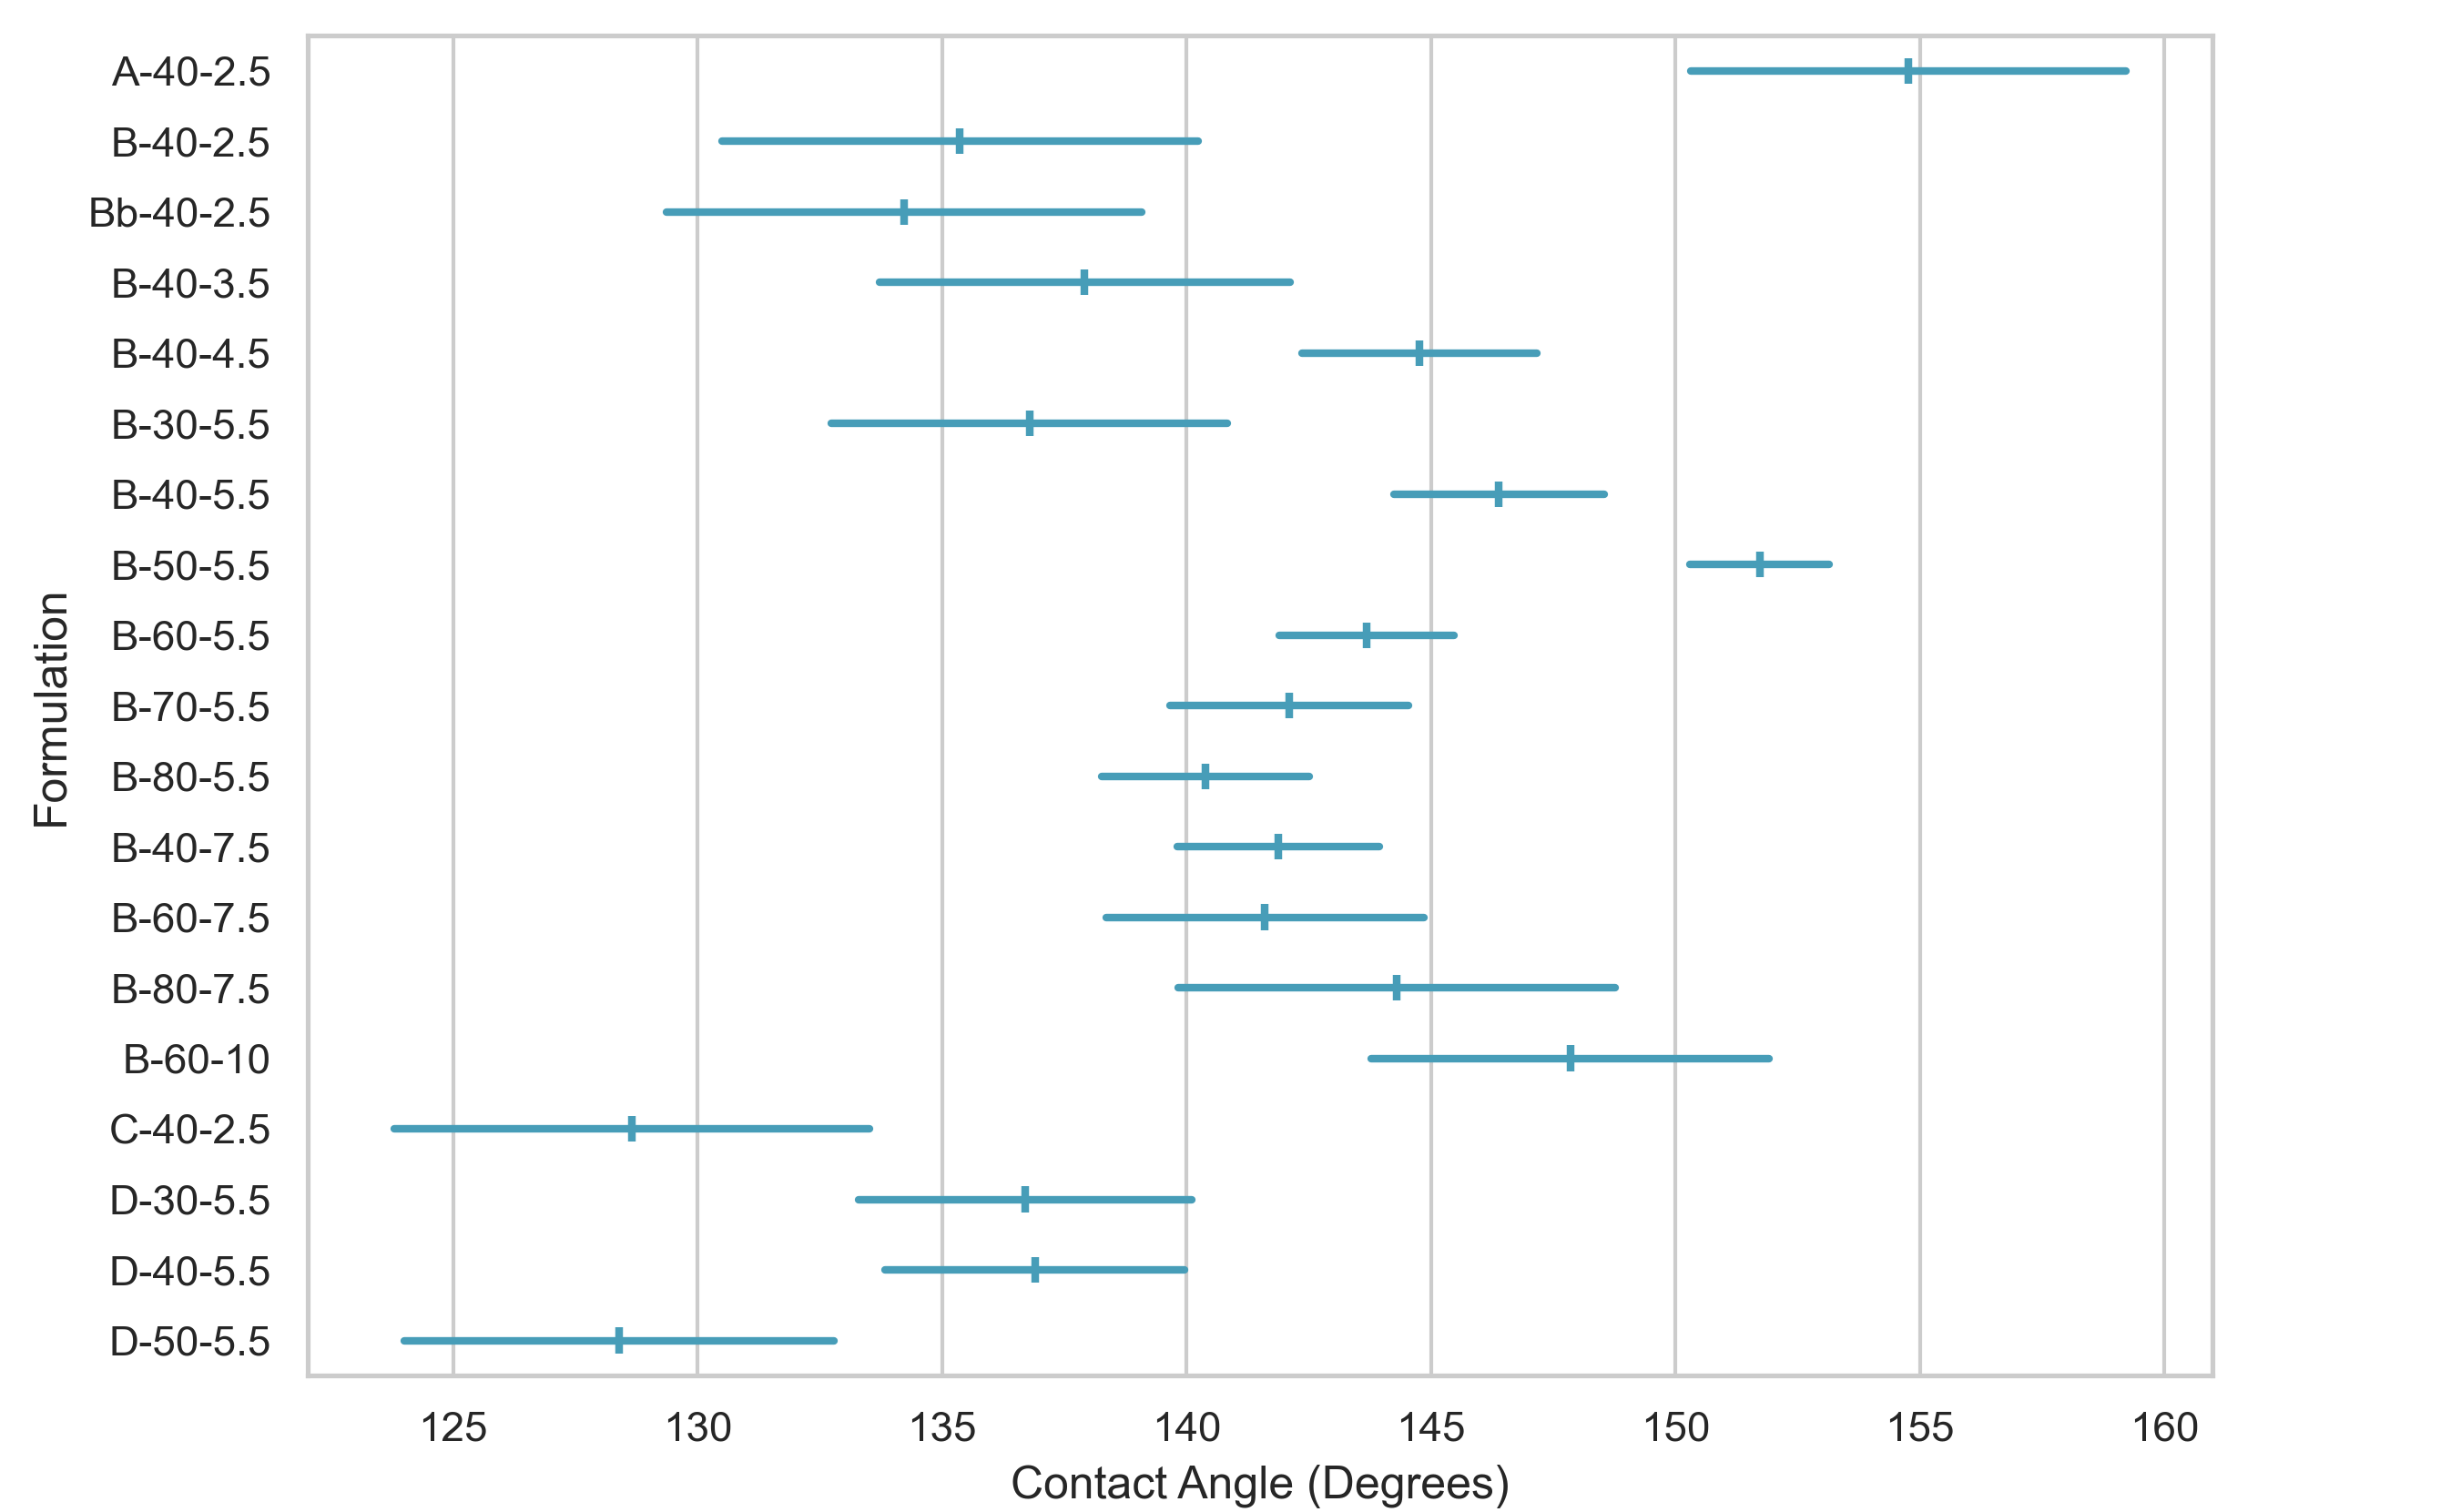
\includegraphics[width=0.523\textwidth]{Sections/Figures/StaticBlue2.png}
  \caption{Static WCA plot for produced formulations presenting mean  \& standard deviation. Films that exhibited absorption are omitted.}\label{CAs}
\end{figure} 

\begin{wrapfigure}{r}{0.2\textwidth}
\centering
    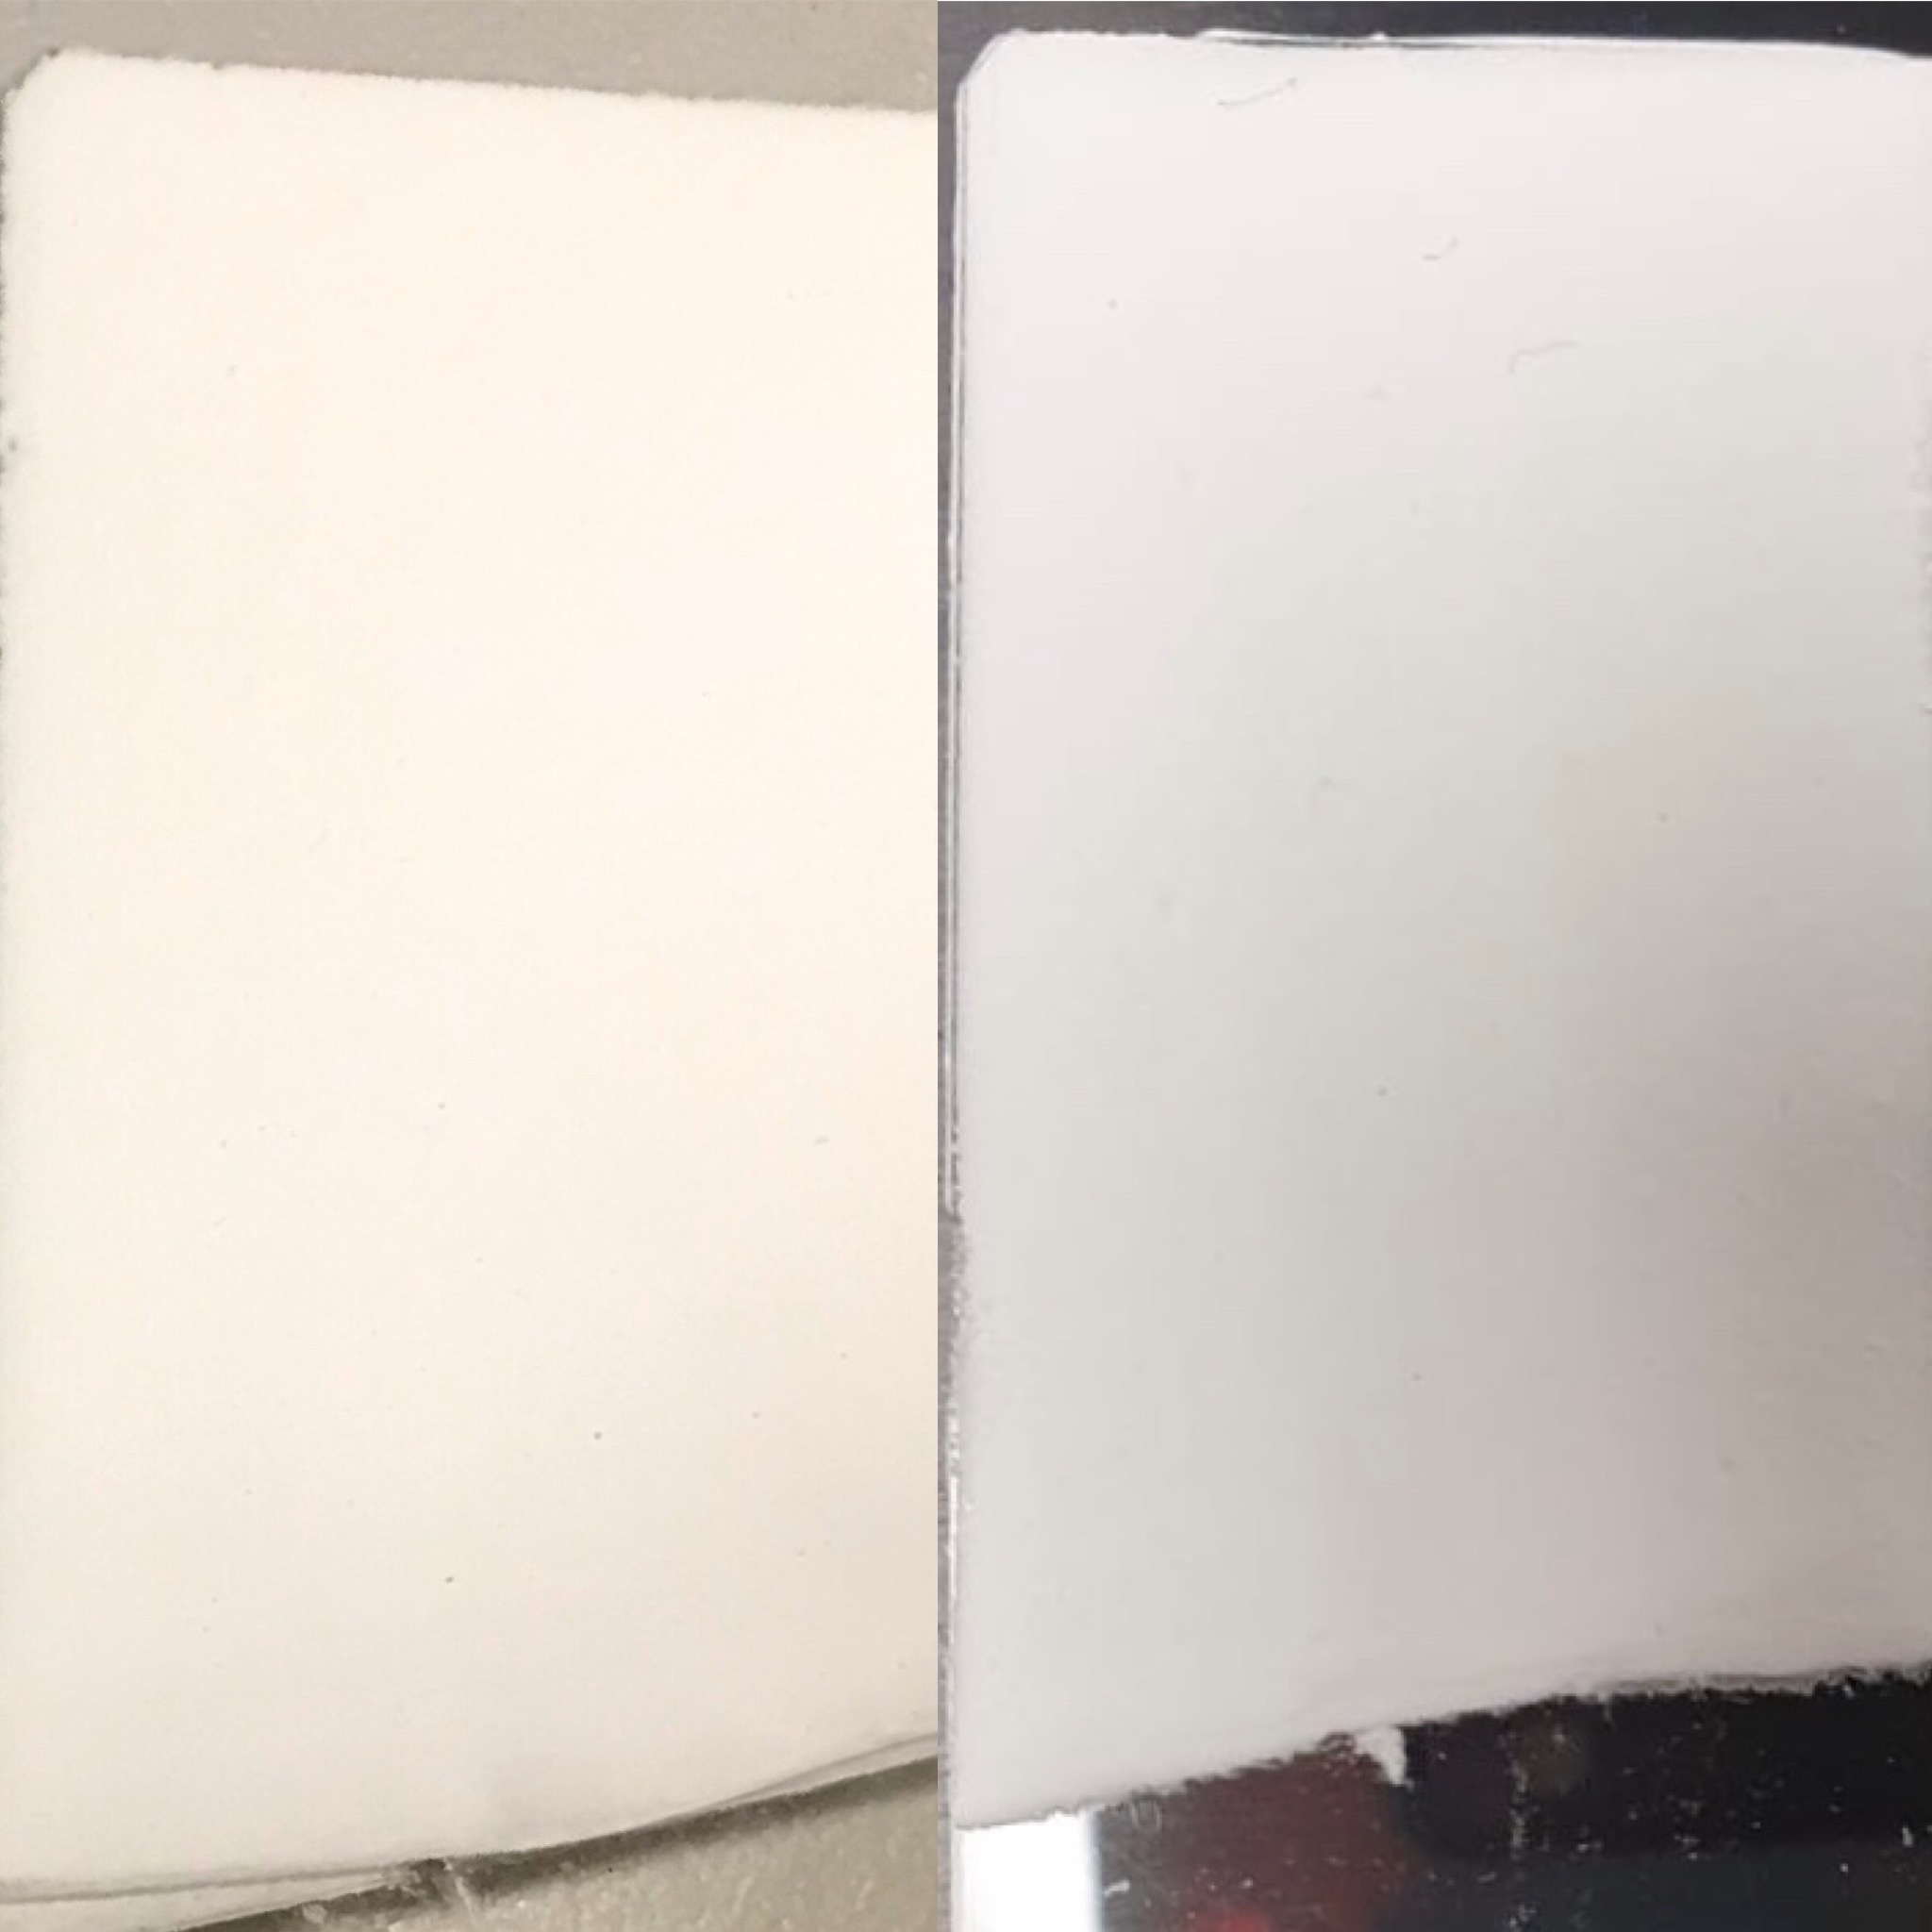
\includegraphics[width=0.1\textwidth]{Sections/Figures/AandB.jpeg}

  \caption{Side by side comparison of A-40-2.5(left) B-50-5.5(right)}
  \label{Comp}
\end{wrapfigure}

Figure \ref{CAs} presents a global view of collected static WCA's; from here it can be concluded that B-50-5.5 is the optimal formulation being statistically higher than all other starch based formulations (bar B-60-10 which exhibited in-homogeneous, powdery and unacceptable film properties). B-50-5.5 overlapped with A-40-2.5, showing comparable static water contact angles.

\begin{wrapfigure}{r}{0.2\textwidth}
\centering
    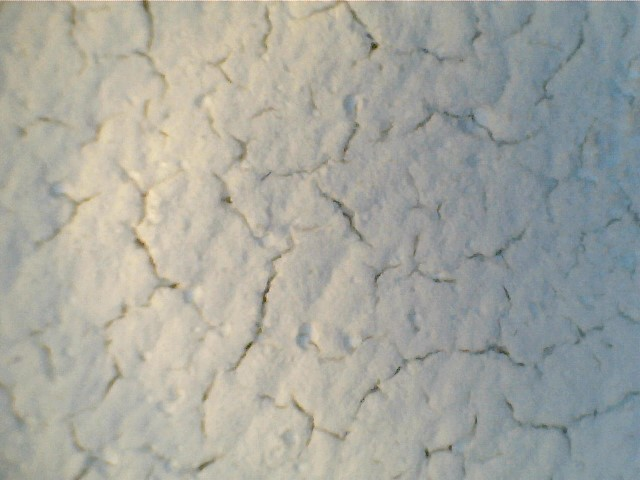
\includegraphics[width=0.1\textwidth]{Sections/Figures/WIN_20201203_13_09_29_Pro.jpg}
  \caption{Bb-40-2.5 image at 25X magnification}
  \label{Bcrack}
\end{wrapfigure}
\par \textbf{Observations} worth noting here were the failure of attempted starch modifications. It was hypothesised that OMS produced a more hydrophobic film (\cite{jiang_dai_qin_xiong_sun_2016}) but exploratory experiments yielded observations of cracking and non-continuous film formation. It is postulated that the increased hydrophobicity of the particles interfered with the gelatinisation process of starch and therefore prohibited optimal dispersion of the OMS in 1:1 DI Water to Ethanol mixture. OMS was not able to be characterised as droplets were absorbed into the surface. TEOS films on the other hand showed improved film forming ability. However, TEOS and the other starch-inorganic hybrid nano-silica (Formulation C), exhibited sub-par hydrophobicity. It is possible that these inorganic silica particles, whether formed from TEOS (\cite{TEOS}) in D or from silica nanoparticles in C interfered with the binding action of starch. 'Bb-40-2.5' was investigated to determine influence of drying rate on WCA. As seen in figure \ref{CAs} there was a 1.5° reduction in static CA compared to the vacuum cupboard dried B-40-2.5 and crack formation was observed due to the increased drying rate as in Figure \ref{Bcrack}.


\subsection{Optimisation of Formulation B}
\begin{figure}[h!]
\centering
  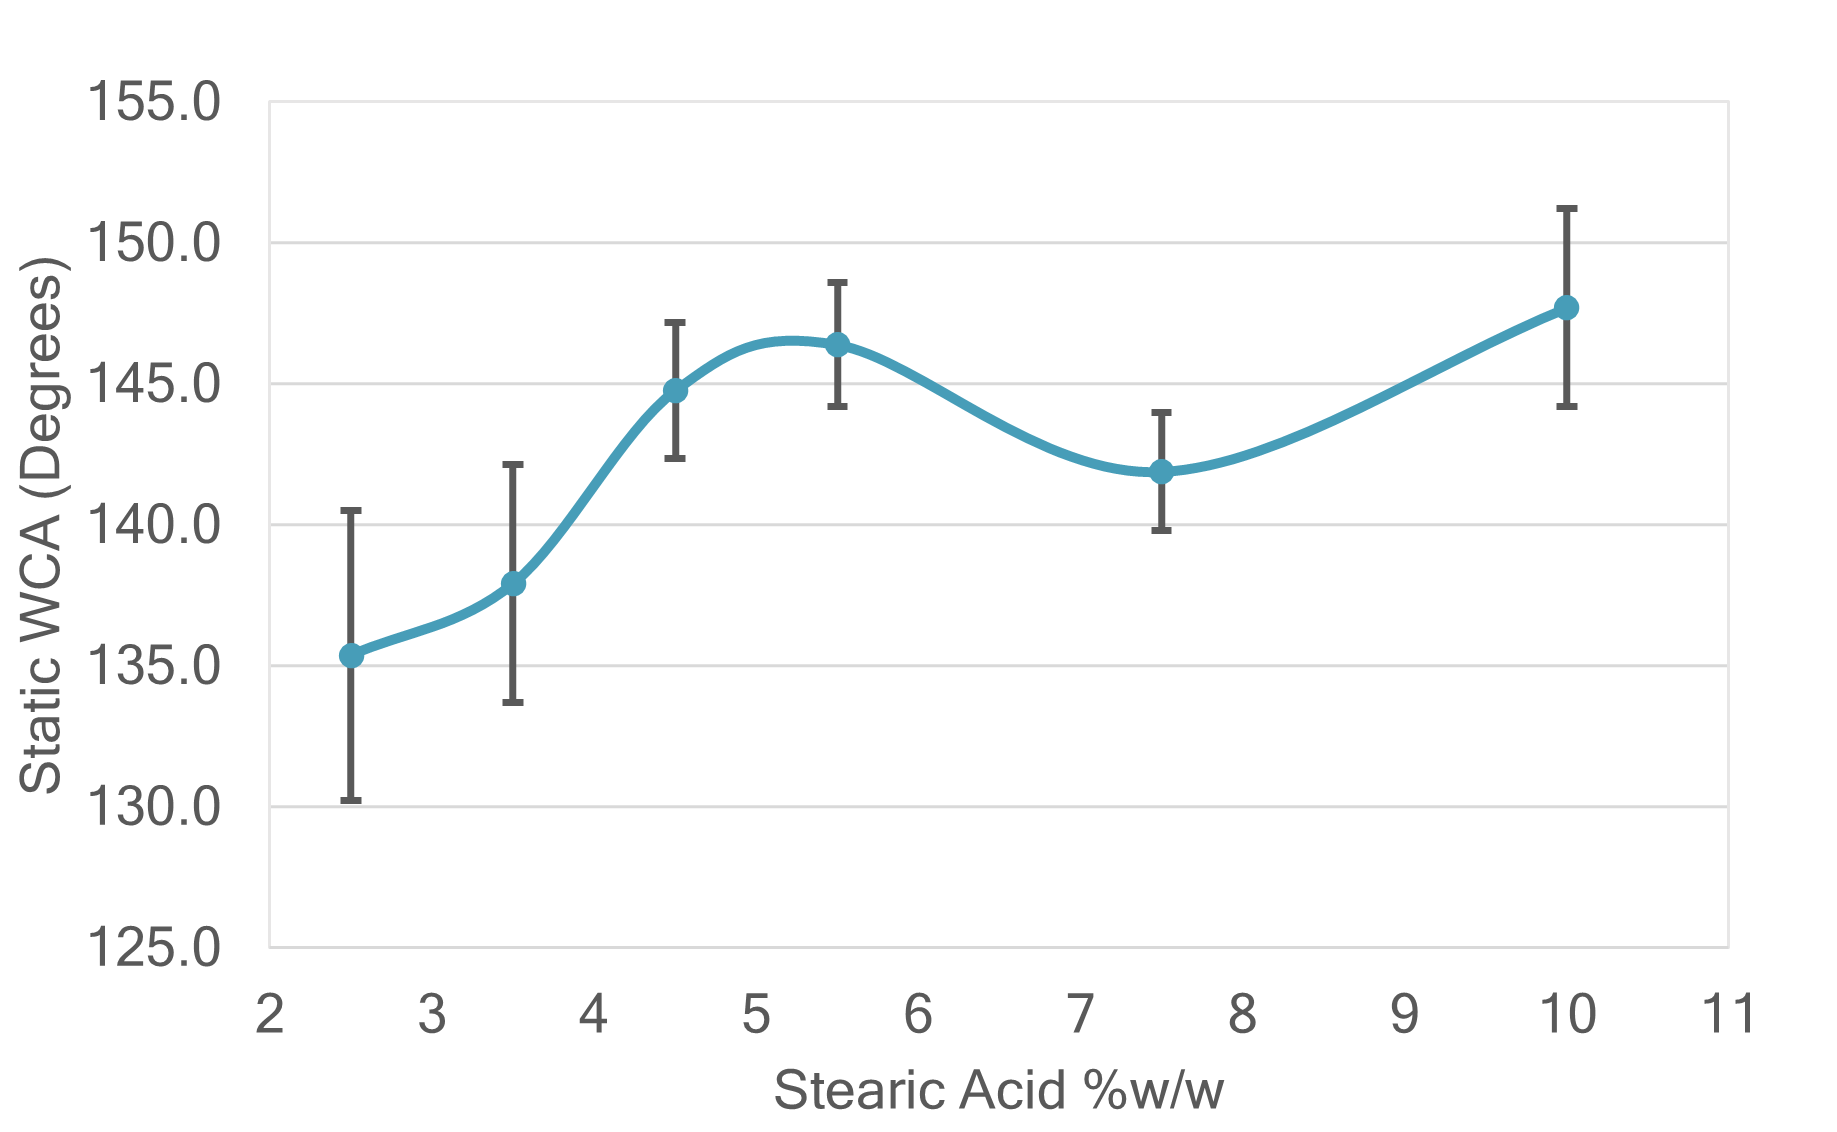
\includegraphics[width=0.4\textwidth]{Sections/Figures/SAOptimise.png}
  \caption{The effect of increasing stearic acid \%w/w for 40\% w/w hydrophobic powder of formulation B}\label{SAOpt}
\end{figure}

As hydrophobic stearic acid (SA) \%w/w was increased, a local maximum was observed; figure \ref{SAOpt} shows that for 40\% w/w SHP, the optimum stearic acid addition content in calcium carbonate was 5.5 \% w/w with a water CA of 146.4° $\pm$ 2.2°. Beyond the optimum, the film became excessively powdery due to physisorbed SA SHP on the calcite surface resulting in a fluctuating WCA with a high SD. Therefore, the optimum was determined at 5.5\%w/w to align with the objective of producing a homogeneous and continuous film. Pure stearic acid has a CA of ~ 120° so it is expected that further increase in SA content will lead to a drop in CA.

\begin{figure}[h!]
\centering
  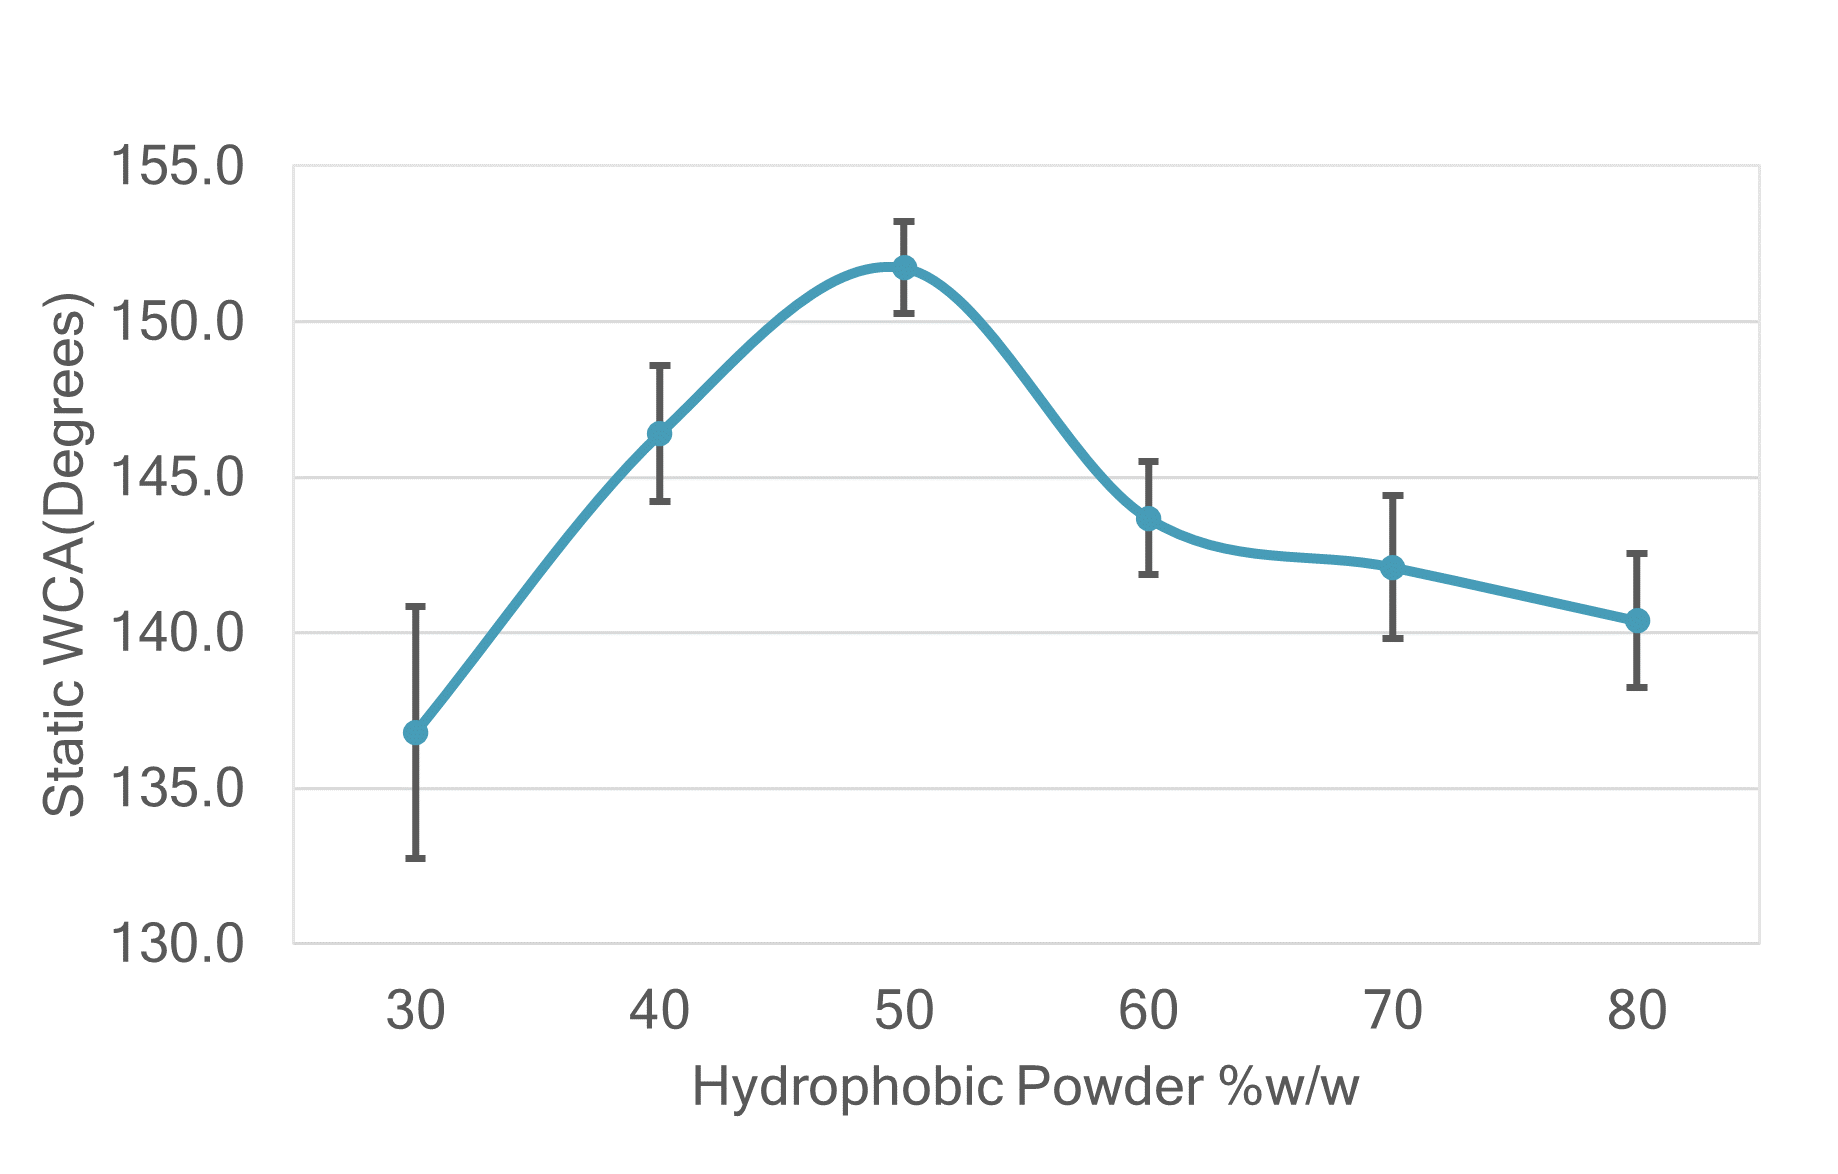
\includegraphics[width=0.4\textwidth]{Sections/Figures/HPOptimise.png}
  \caption{The effect of increasing hydrophobic powder content for 5.5\%w/w stearic acid of formulation B }\label{HPOpt}
\end{figure}

Figure \ref{HPOpt} shows that for a SA weight \% of 5.5, the optimum addition of SHP was 50\%w/w with a WCA of 151.7 $^\circ$ $\pm$ 1.5. Increasing SHP content improved hydrophobicity and viscosity for adhesion during dip coating. However, there was a compromise; as the binding solvent became more saturated there was a corresponding increase in in-homogenous film formation which featured pockets of non-bound powder. An optimum was therefore chosen to avoid this.   


\subsection{Receding Contact Angle}
Measuring $\theta_R$ using the sessile drop method led to considerable difficulty due to the rough surface topography of the samples. The droplet did not recede when water was withdrawn via the needle as the contact line remained pinned. This was ascribed to the local defect mechanism (\cite{hong_chang_chou_chan_sheng_tsao_2011}); the presence of local defects that were considerably more wettable than the rest of the surface. Instead of receding, the withdrawal of the water caused a change of the droplet shape from a spherical cap to a conical one as demonstrated by figure \ref{Cone}. This effect was enhanced through the adhesion of water to the hydrophilic steel needle.   
\par When even more water was withdrawn, the water snapped away from the needle. This indicated that the adhesion between the water and the films being analysed was higher than the cohesion between water molecules. Due to these reasons, $\theta_R$ could not be measured on any of our samples using this method. 



\begin{figure}[h!]
\centering
  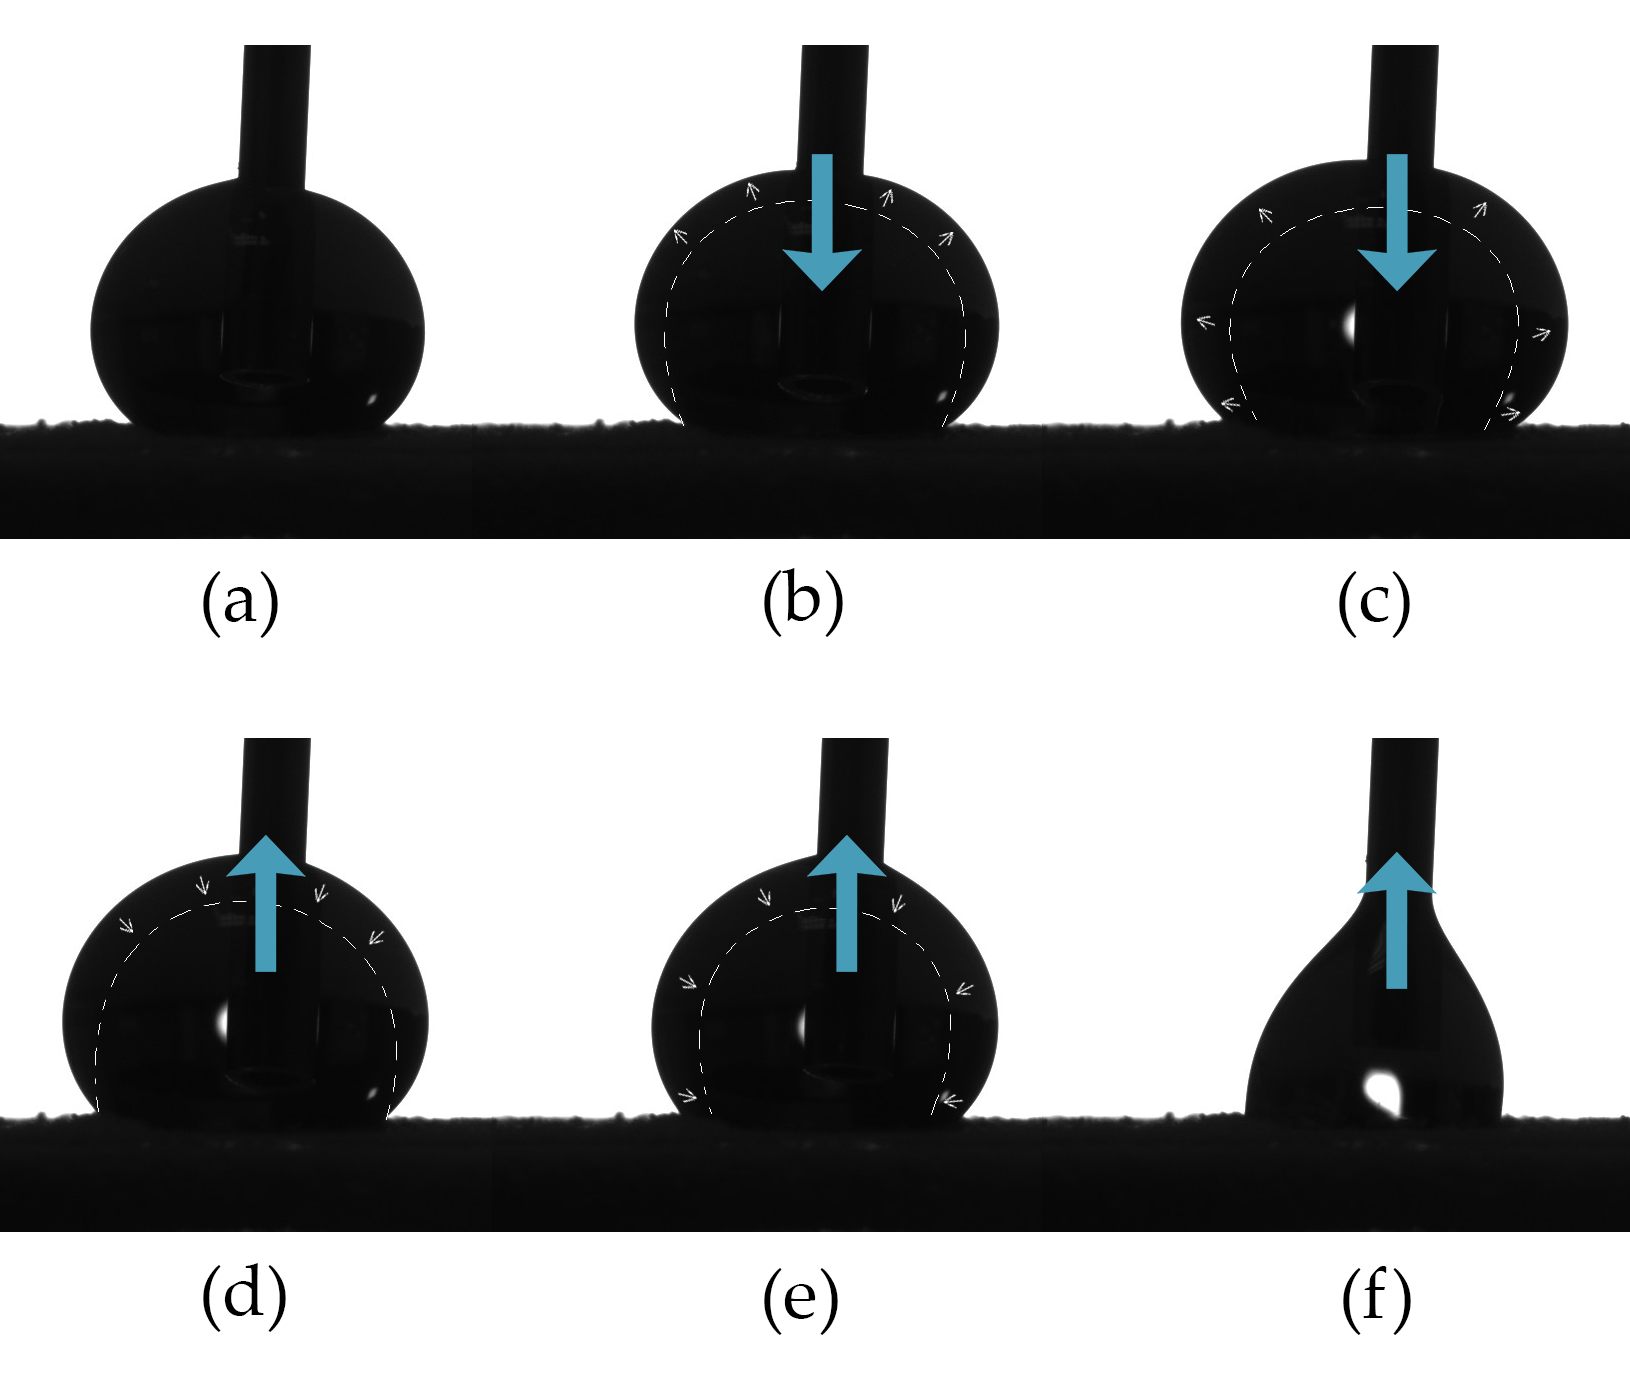
\includegraphics[width=0.45\textwidth]{Sections/Figures/sessile3.png}
  \caption{Photograph sequence showing the sessile-droplet method with receding contact line pinning on a formulation C slide\footnotemark: (a) The initial droplet volume ($20\mu L$); (b) Volume dispense increment before contact line advancement; (c) contact-line advancement due to volume increments dispensed into droplet; (d) reduction in droplet volume before droplet starts receding (with a pinned contact line); (e) A suction increment showing a receding contact line; (f) Further reduction in volume with a pinned contact line on slide surface showing the conical-esque shape.}\label{Cone}
\end{figure} 
\footnotetext{Formulation C was chosen for figure 2 as the transition to a conical shape was more apparent and extreme on this film}
\newpage
\subsection{Statistical Analysis of $\theta_A$}
%Contact Angle Measurements}
\begin{figure}[h!]
\centering
  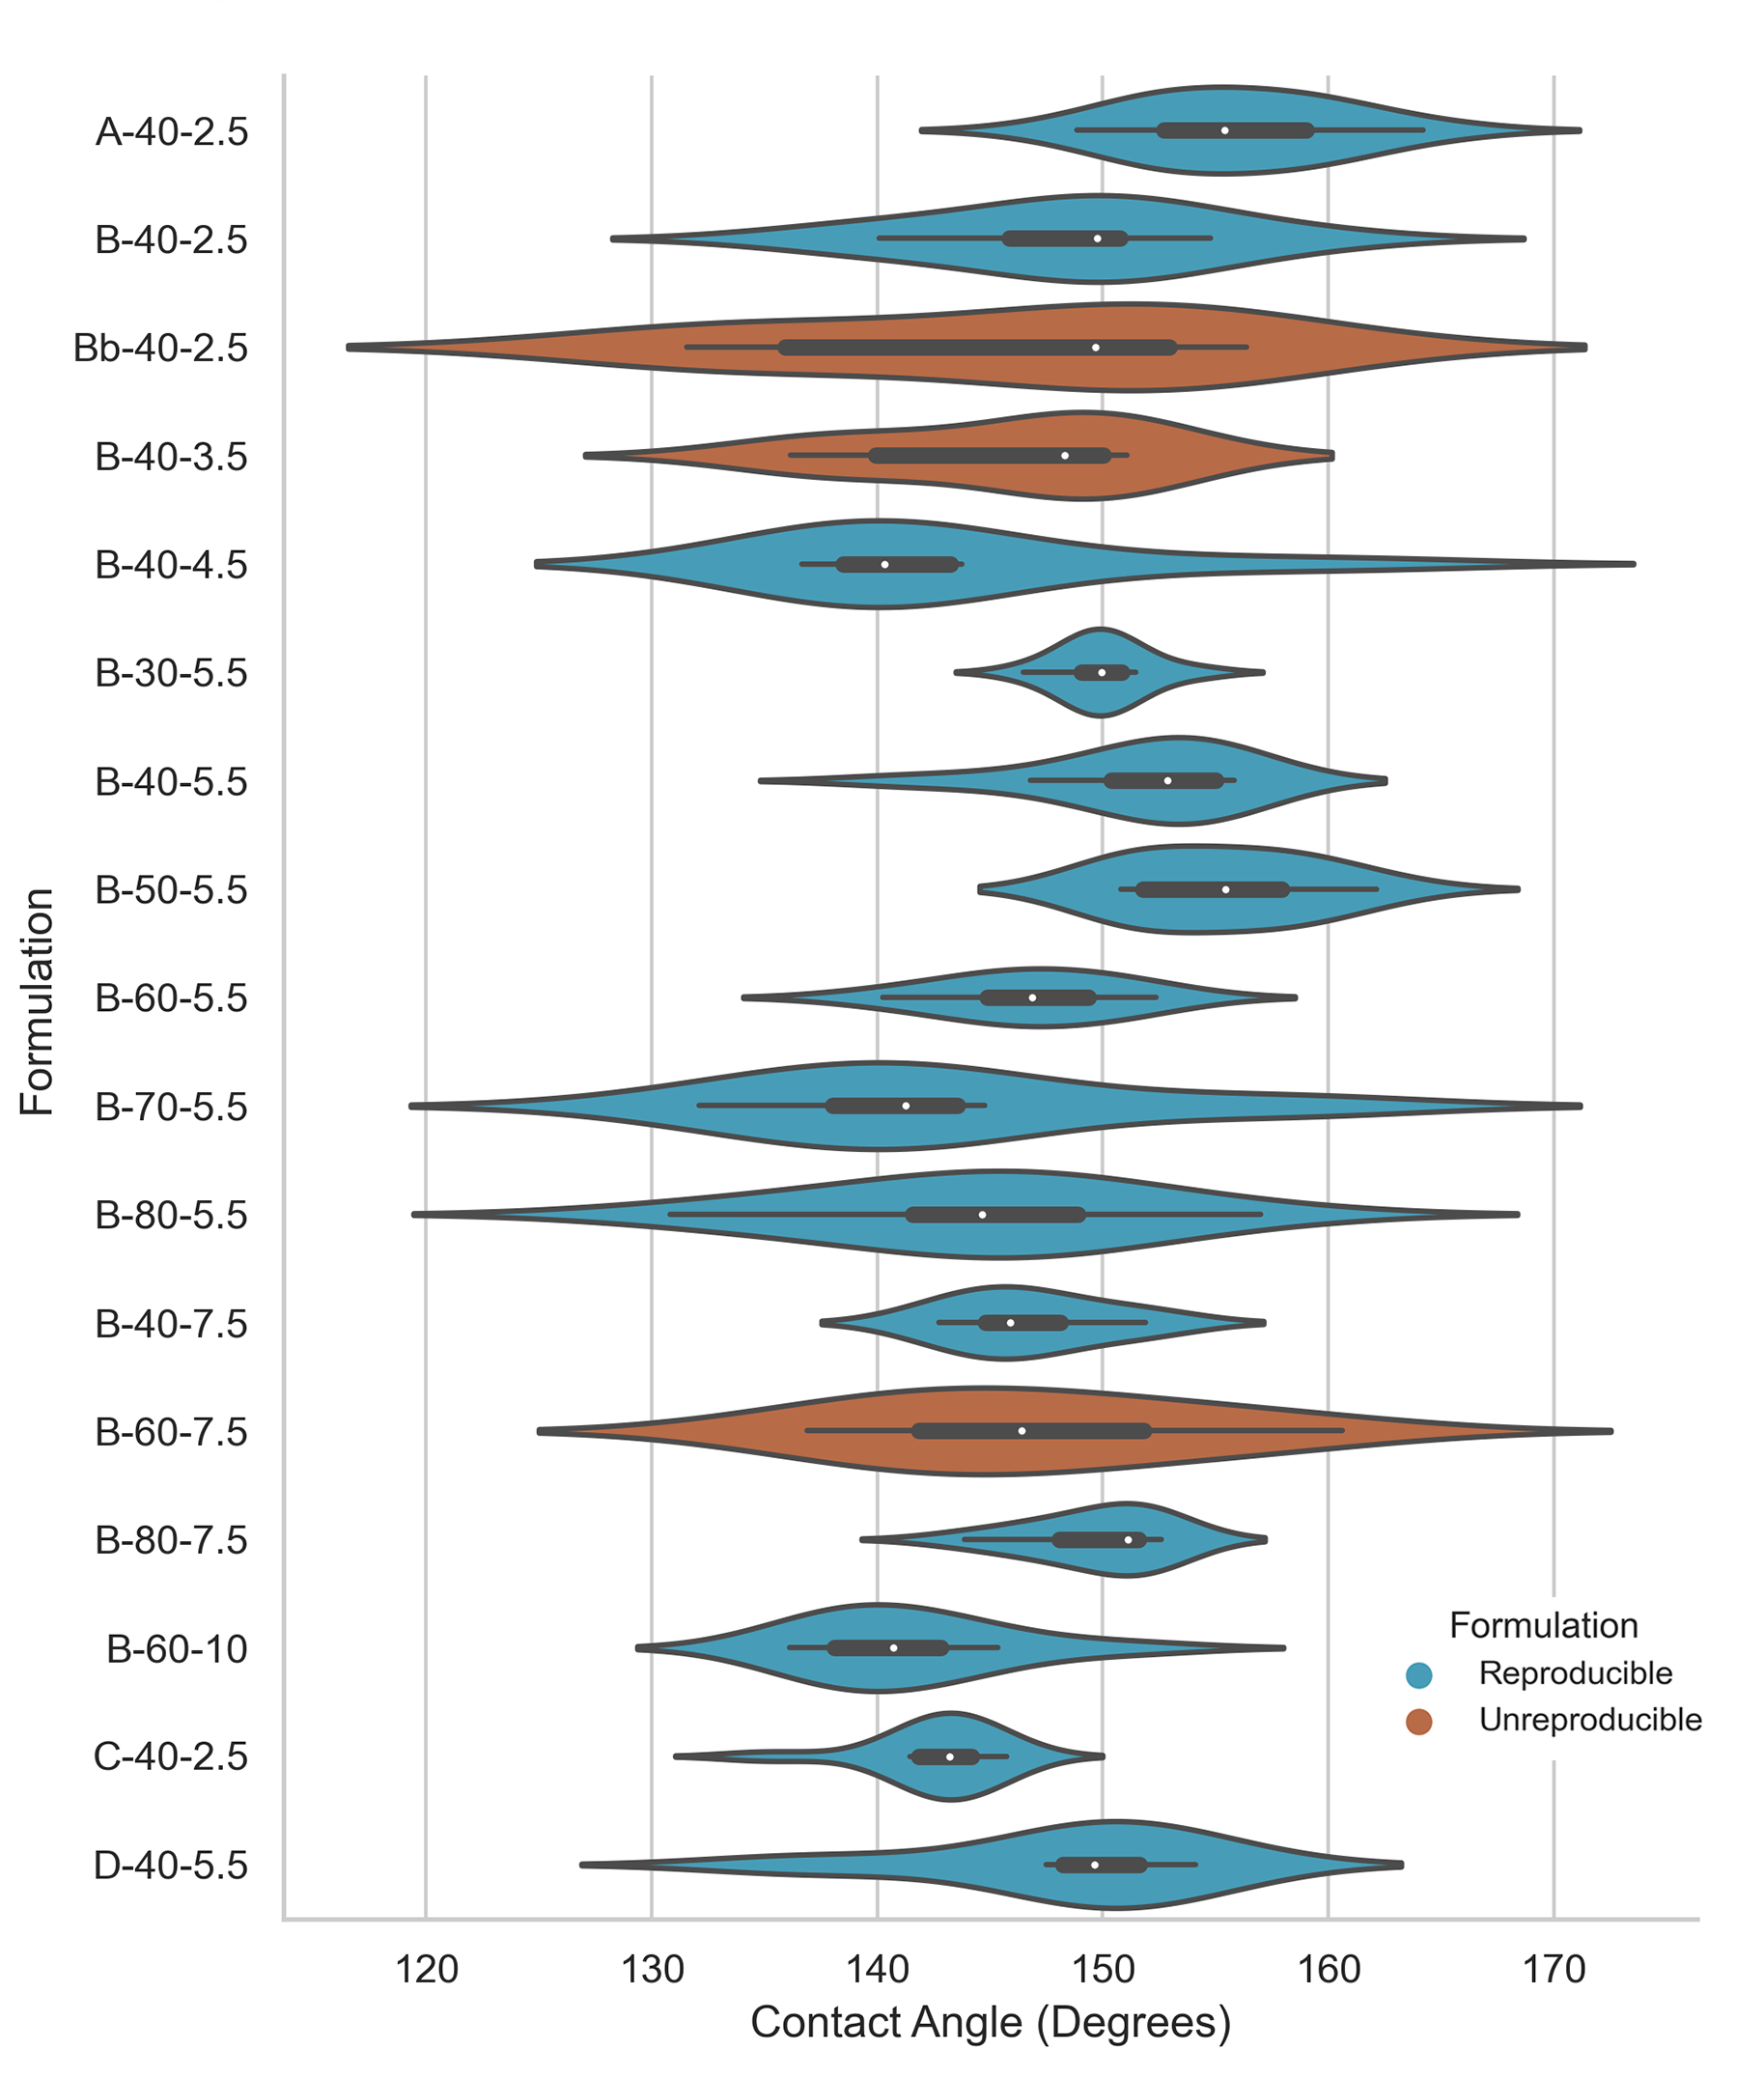
\includegraphics[width=0.5\textwidth]{Sections/Figures/tiny.png}
  \caption{Violin plot of $\theta_A$ for each formulation alongside box and whisker plots. Violin shape is a  kernel density estimation of the underlying $\theta_A$ distribution.}\label{CA}
\end{figure} 

Figure \ref{CA} depicts the advancing contact angle measurements, which were all achieved with well fitting polynomials with a mean $R^2$ value of 0.99 from all experiments, indicating excellent goodness-of-fit. 
\par During intra-formulation slide-to-slide analysis of $\theta_A$, a P value of $x$ can be understood as an $x\%$ likelihood that the difference in means was due to random chance. Conventionally, a P value < $\alpha = 0.05$ is significant in which case we rejected the null hypothesis, $H_0:\mu_1 = \mu_2$.  If the P value was greater than 0.05, we do not reject the null hypothesis and concluded no statistical significant difference between the two slides. 
\par The only formulations that exhibited statistically significant differences between slides within the 95\% confidence interval were Bb-40-2.5, B-40-3.5 \& B-60-7.5 as shown in Figure \ref{CA} as 'unreproducible'. For the remaining formulations, it can be assumed that dip coating played an insignificant role in variance. Data can be safely grouped together and analysed as the remaining possible causes of formulation variance are chance and surface in-homogeneity. The interquartile range (IQR) for each formulations is presented in figure \ref{CA} and is an indicator of surface homogeneity for each film, with outliers accounted for. It was concluded that all reproducible films showed comparable surface homogeneity, attesting to the viability of a starch superhydrophobic films.
\par The null hypothesis \emph{between} the starch-based film formulations was that of identical means ($H_0: \mu_A = \mu_B = \mu_C =...$). ANOVA was carried out on all starch-based films. With a calculated F-statistic and F crit of $4.560159>1.699042$ respectively, the null hypothesis was rejected and it was concluded that at least one of the formulations exhibited statistical difference. Since this was simply an 'omnibus' test, further t-testing was performed to investigate pair-wise statistical differences between formulations; namely B-50-5.5. B-50-5.5 was statistically different when compared to B-40-5.5 with a 95\% likelihood, and statistically different to all other formulations with at \emph{least} a 99.5\% liklihood. B-50-5.5, the optimised formulation, therefore features statistically superior $\theta_A$'s to the other starch formulations.
\par Conversely, with a p-value of $0.6695104>0.05$, the null hypothesis $H_0: \mu_B_-_5_0_-_5_._5 = \mu_A_-_4_0_-_2_._5$ could not have been rejected. The measured $\theta_A$'s for B-50-5.5 and A-40-2.5 were \emph{not} statistically different. This leads again to the conclusion that starch at 5.5\% w/w SA and 50\% w/w functionalised powder is a viable replacement for toluene and PE as presented by \cite{khoo_lim_2017}. The films exhibited comparable super hydrophobic contact angles and surface homogeneities (IQR's) as shown in figure \ref{CA}.



\subsection{Durability Characterisation}
\begin{figure}[H]
\centering
\begin{subfigure}{.22\textwidth}
%  \centering
  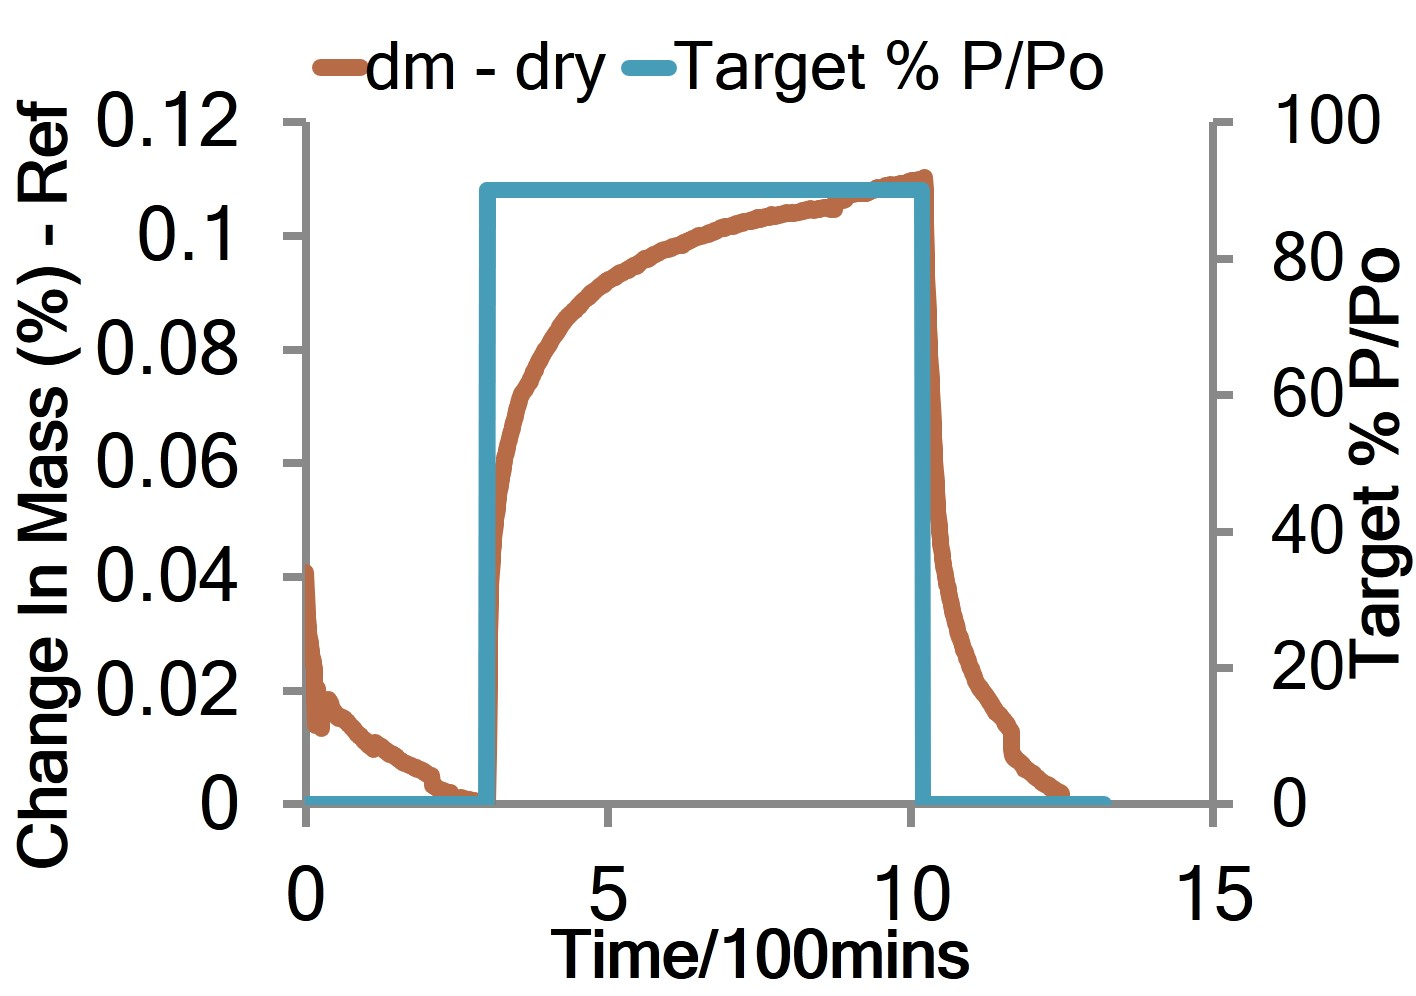
\includegraphics[width=1\linewidth]{Sections/Figures/DVSA.jpg}
  \caption{A-40-2.5}
  \label{fig:sub1}
\end{subfigure}
%.48 before
\begin{subfigure}{.22\textwidth}
%  \centering
  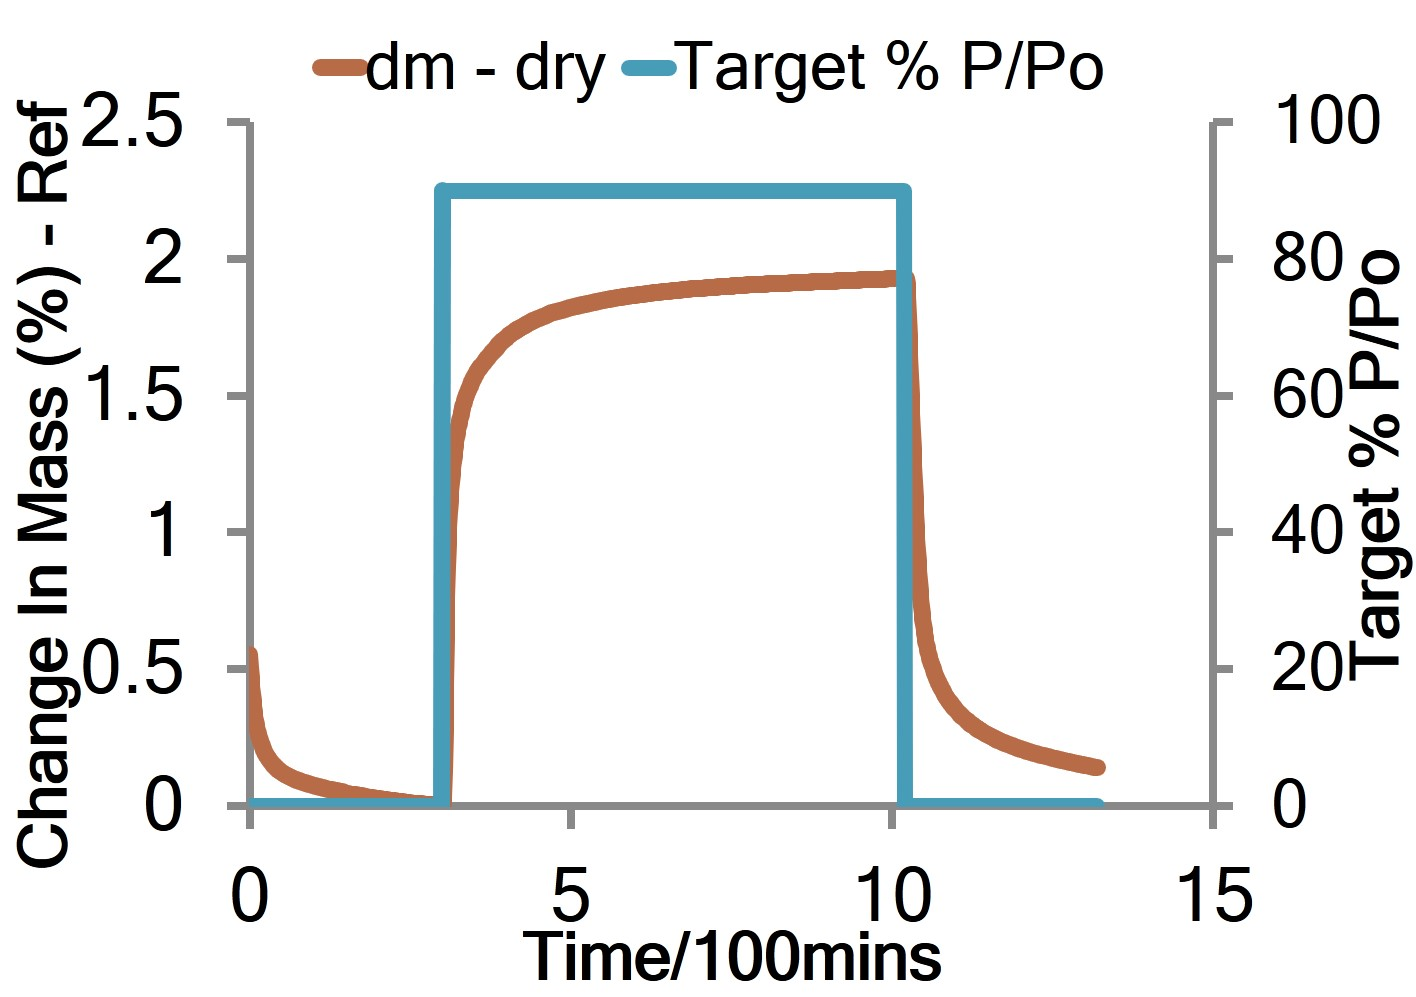
\includegraphics[width=1\linewidth]{Sections/Figures/DVSB.jpg}
  \caption{B-50-5.5}
  \label{fig:sub2}
\end{subfigure}
\caption{DVS Advance traces taken at 24.7 °C}
\label{fig:test}
\end{figure}

\textbf{DVS experiments} were completed allowing sufficient time for plateaus at 90\% RH. It has been concluded that 'B-50-5.5' is 17.5x more hygroscopic than 'A-40-2.5'. It was promising however that 'B-50-5.5' is 8x less hygroscopic than native corn starch. The higher hygroscopicity is due to the inherent hydrophilicity of the hydroxyl groups on starch polymers. Smaller step changes can be used to determine a potential type ii isotherm (\cite{starch_dvs}). 
\par \textbf{Immersion tests} studied the formulation’s hydrophobic durability while the slides were in prolonged contact with water. From visual observations, upon immersion the surface became reflective (Figure \ref{silver}) as a result of a pinned air layer, characteristic of a superhydrophobic coating in the Cassie Baxter regime, as mentioned.  When slides were removed, the surface appeared dry regardless of drying with compressed N$_2$. 

\begin{wrapfigure}{l}{0.2\textwidth}
\centering
    \includegraphics[width=0.1\textwidth]{Sections/Figures/silver.png}
  \caption{Reflection on an A-40-2.5 slide resulting from pinned air layer}
  \label{silver}
\end{wrapfigure}



%\begin{figure}[h!]
%\centering
%  \includegraphics[width=0.15\textwidth]{Sections/Figures%/silver.png}
%  \caption{Reflection on an A-40-2.5 slide resulting from %pinned air layer}\label{silver}
%\end{figure}




\begin{figure}[h!]
\centering
  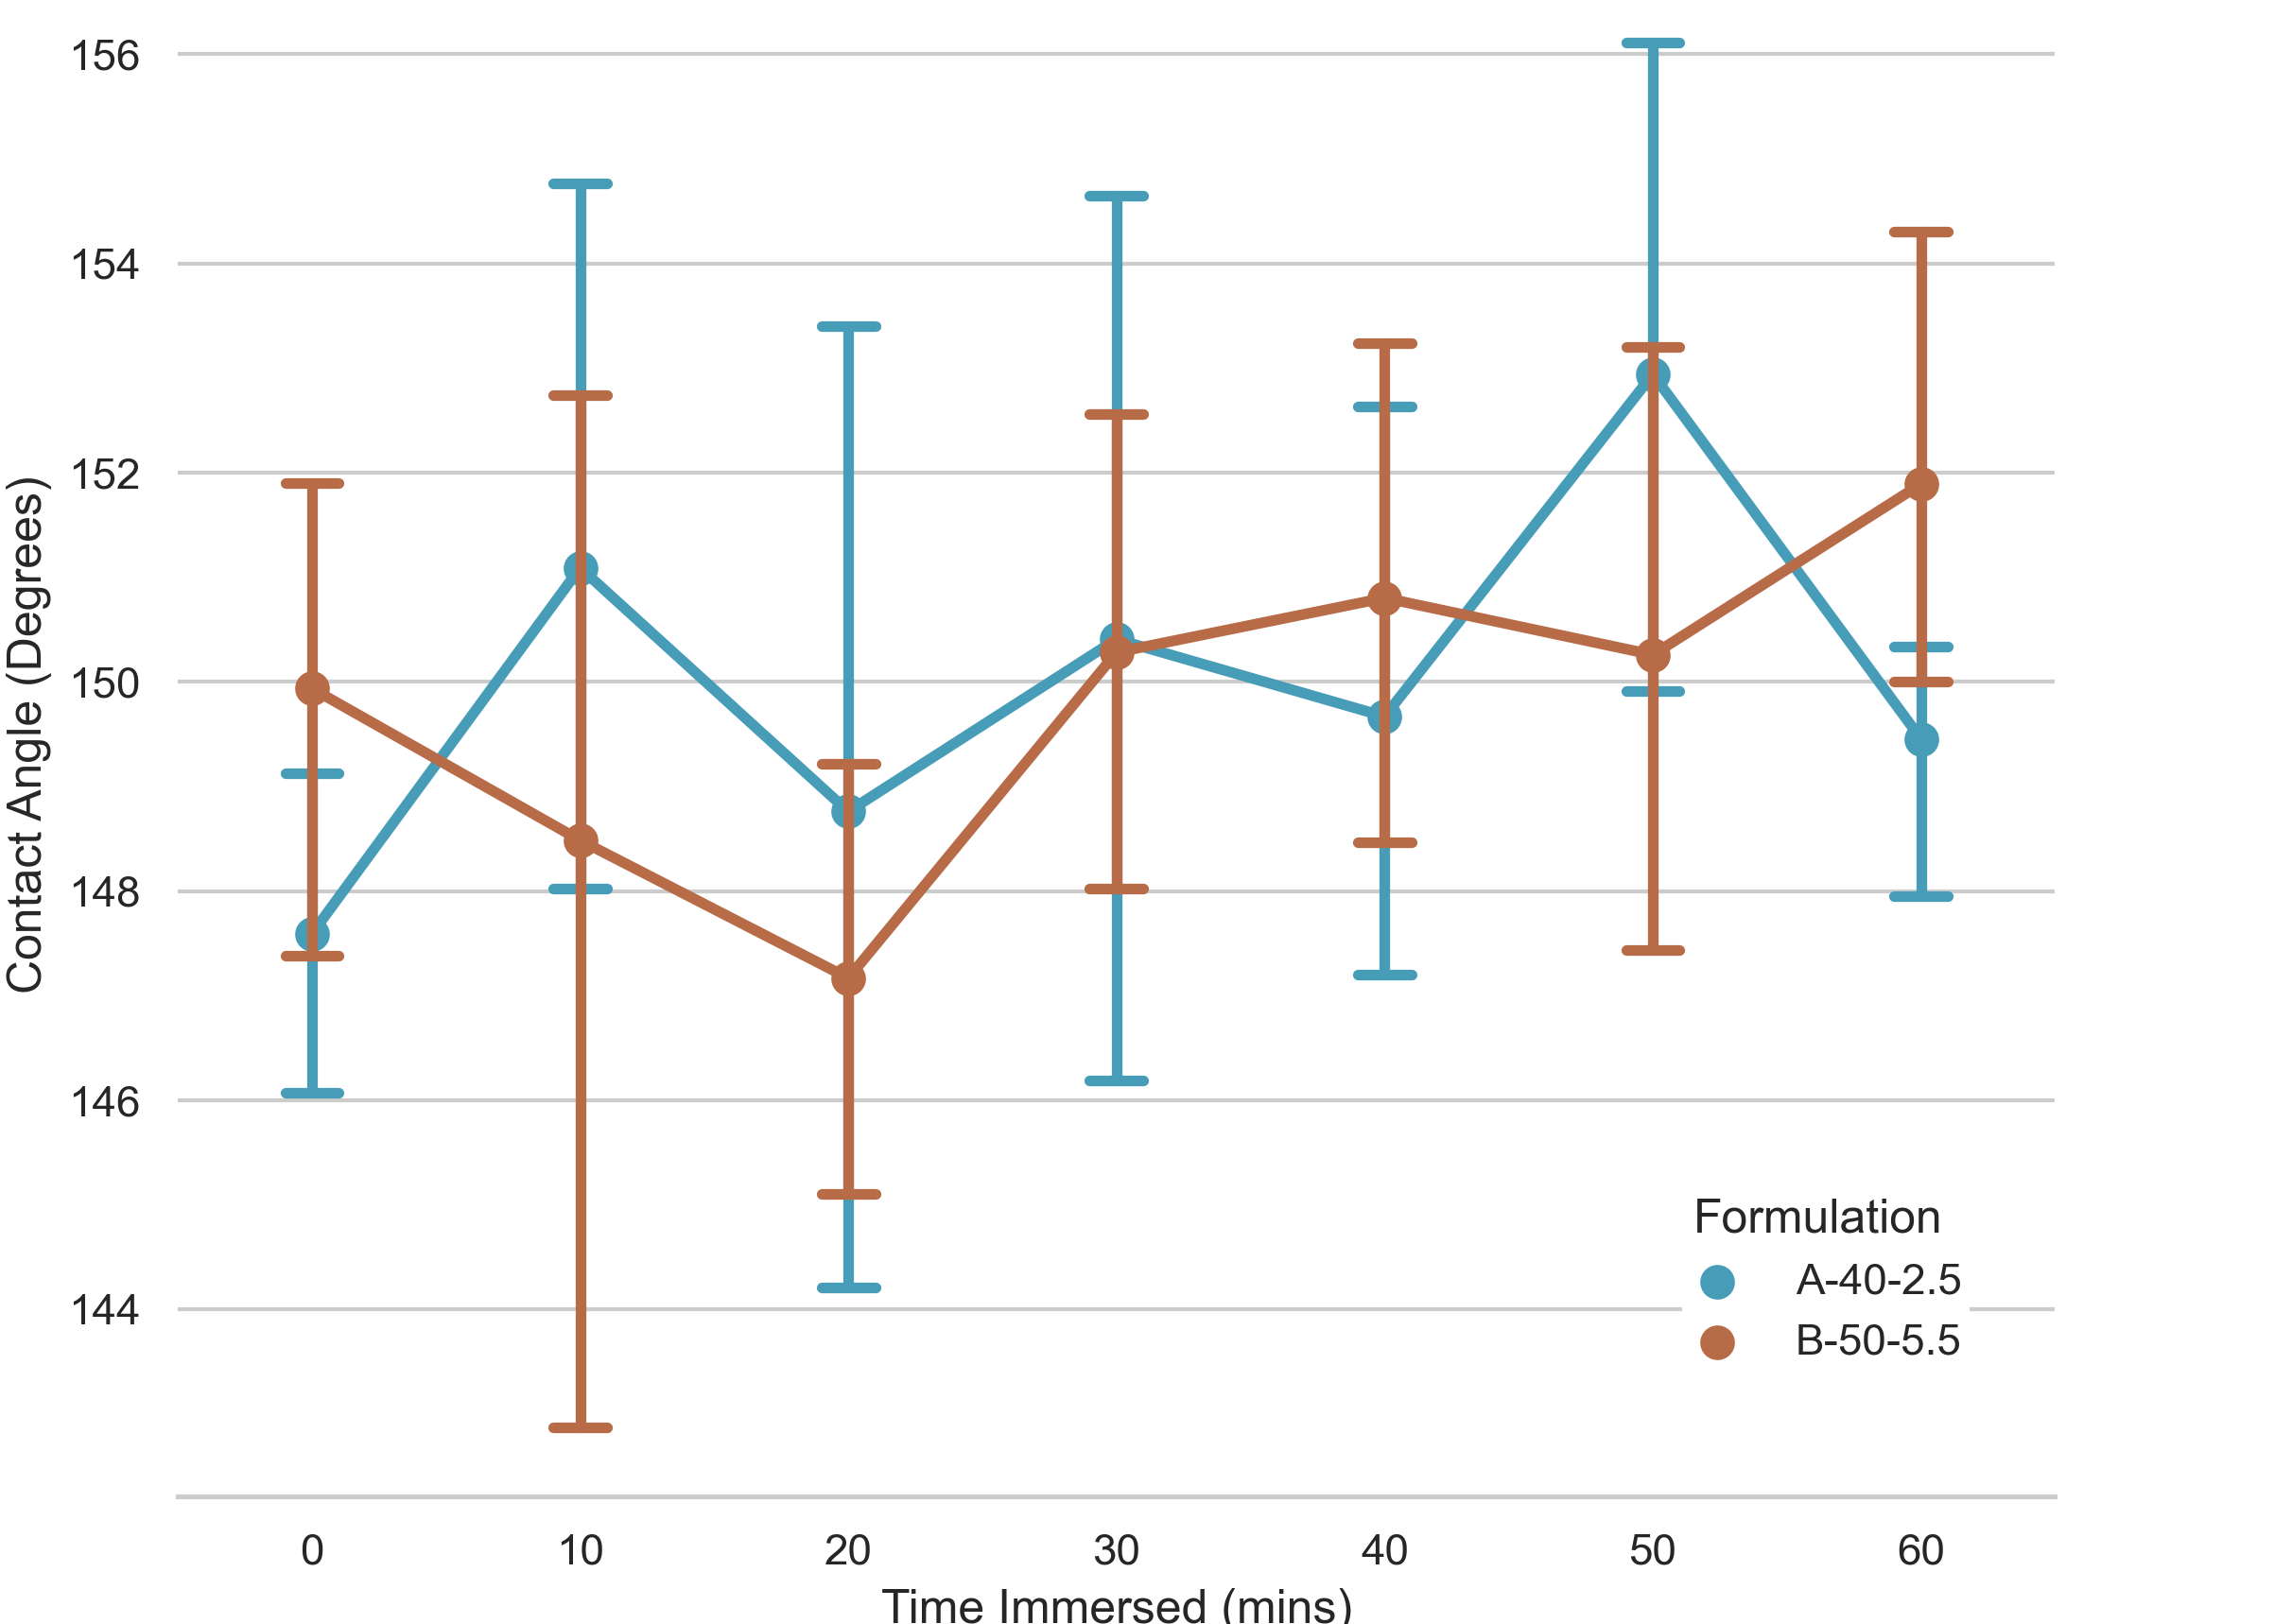
\includegraphics[width=0.43\textwidth]{Sections/Figures/Immersion3.png}
  \caption{Plot of Contact Angle as a function of time immersed in water for PE/Toluene and optimised formulation, showing standard deviation bars}\label{Immersion}
\end{figure} 
Figure \ref{Immersion} demonstrates that there was no statistically significant drop in hydrophobicity for either of the slides due to an overlap in the standard deviation bars. In addition, the formulations show no statistical difference \emph{between} each other at any time stamp. This further corroborates the conclusion that B-50-5.5 is a valid replacement for A in terms of super hydrophobicity and durability. 
\\ 
\par Nonetheless, a longer immersion time would be insightful as to the long-term effects of immersion. It can be concluded that both the B-50-5.5 and A-40-2.5 coatings show excellent hydrophobic durability up to 1 hour, with no statistically significant degradation,  however long term experiments are required to examine if a plateau has truly been reached. 

\begin{figure}[H]
\centering
\begin{subfigure}{.11\textwidth}
  \centering
  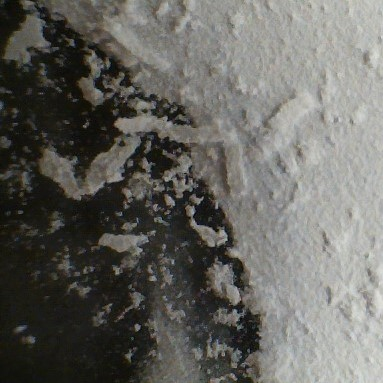
\includegraphics[width=1\linewidth]{Sections/Figures/A_Opt.jpg}
  \caption{A-40-2.5}
  \label{fig:sub1}
\end{subfigure}%
\begin{subfigure}{.11\textwidth}
  \centering
  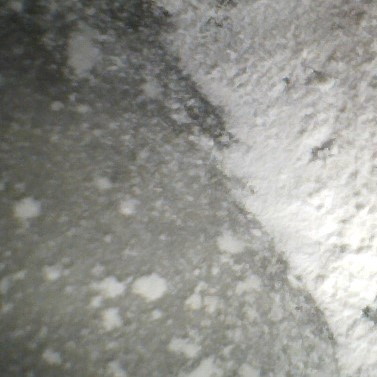
\includegraphics[width=1\linewidth]{Sections/Figures/B_opt.jpg}
  \caption{B-50-5.5}
  \label{fig:sub2}
\end{subfigure}
\caption{Images taken at 50X magnification}
\label{fig:test}
\label{abrased}
\end{figure}
\newpage

\par The average time recorded during \textbf{Mechanical Abrasion Testing} for 2 slides of 'A-40-2.5' and 'B-50-7.5' was 5.1 seconds and 5.7 seconds respectively. The disparity of 0.6 seconds suggests durability is comparable. Figure \ref{abrased} shows that A-40-2.5 formed a more coarse powder due to PE polymer grains. 
\par During \textbf{outdoor testing} 2 Slides of A-40-2.5 and 2 slides of B-50-5.5 were placed on the windowsill from 02-Dec-2020 to 07-Dec-2020 in SW7, London, UK. The average temperature was 5 °C $\pm$ 3°C with an RH of 90\%. Rain was recorded on 3 of the 5 days. 


%\begin{figure}[h!]
%\centering
%  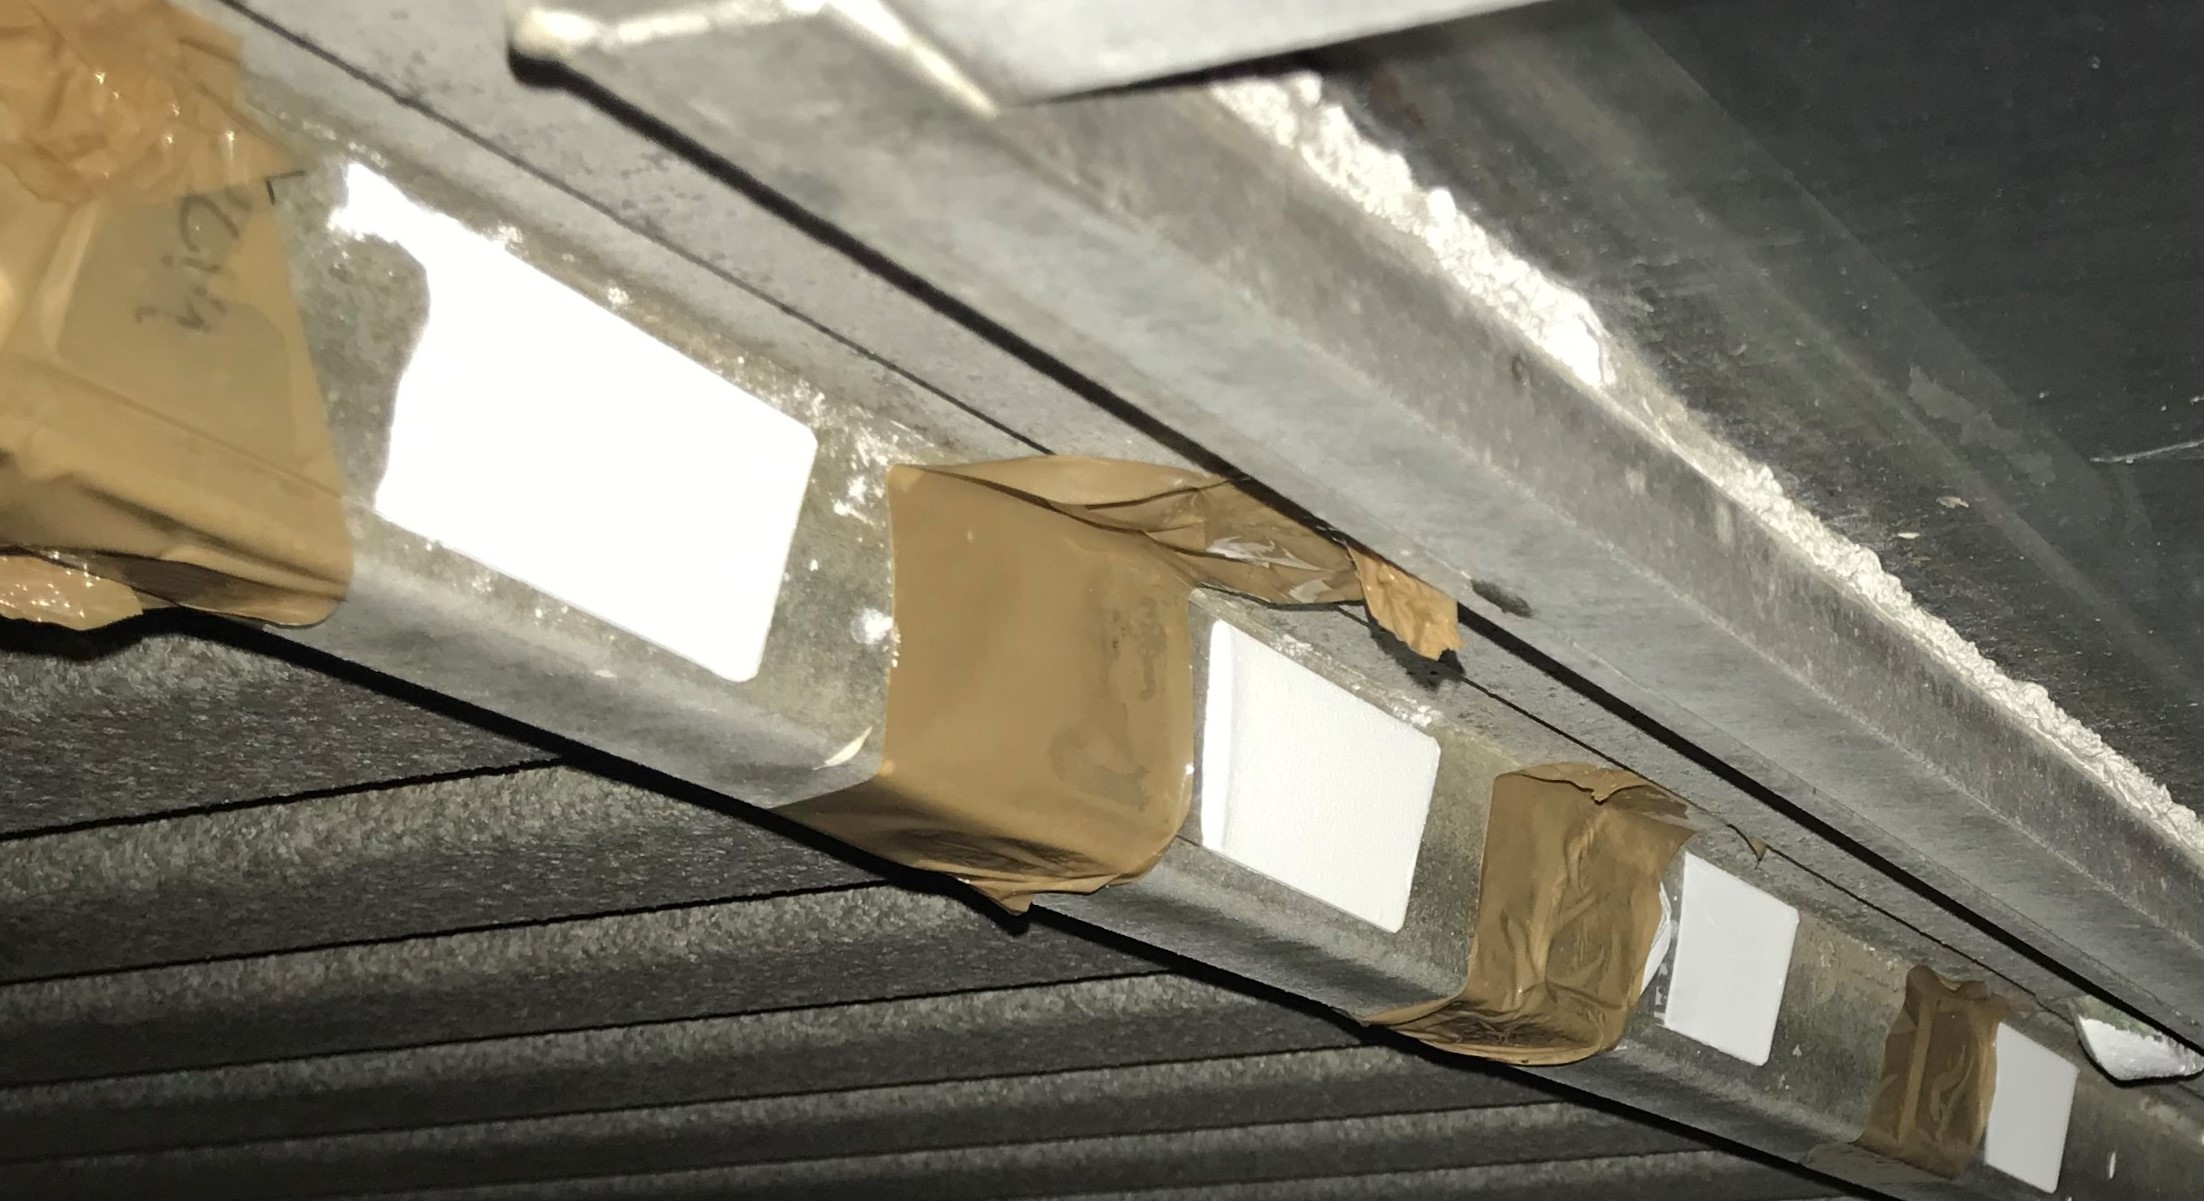
\includegraphics[width=0.2\textwidth]{Sections/Figures/Outdoor2.jpg}
%  \caption{The slides after 5 days of outdoor exposure on the windowsill with B-50-5.5 in the foreground of the image }\label{HPOpt}
%\end{figure}



\begin{table}[H]
\centering
\begin{tabular}{llr111}
\toprule


Description  & $\mu_1$    & $s_1$  & $\mu_2$    & $s_2$  & $t$   \\
\midrule
A-40-2.5 (1) & 152.8 & 3.9 & 147.6 & 1.9 & 2.0 \\ 
A-40-2.5 (2) & 150.1 & 1.1 & 149.7 & 1.1 & 0.4 \\ 
B-50-5.5 (1) & 151.8 & 2.9 & 146.5 & 3.6 & 1.9 \\ 
B-50-5.5 (2) & 151.6 & 1.8 & 150.9 & 2.5 & 0.4 \\ 
\bottomrule
\end{tabular}
\caption{1 is before and 2 is after the outdoor test. $\mu$ is the mean static WCA and $s$ is the sample standard deviation}
\end{table}
\begin{wrapfigure}{r}{0.23\textwidth}
\centering
    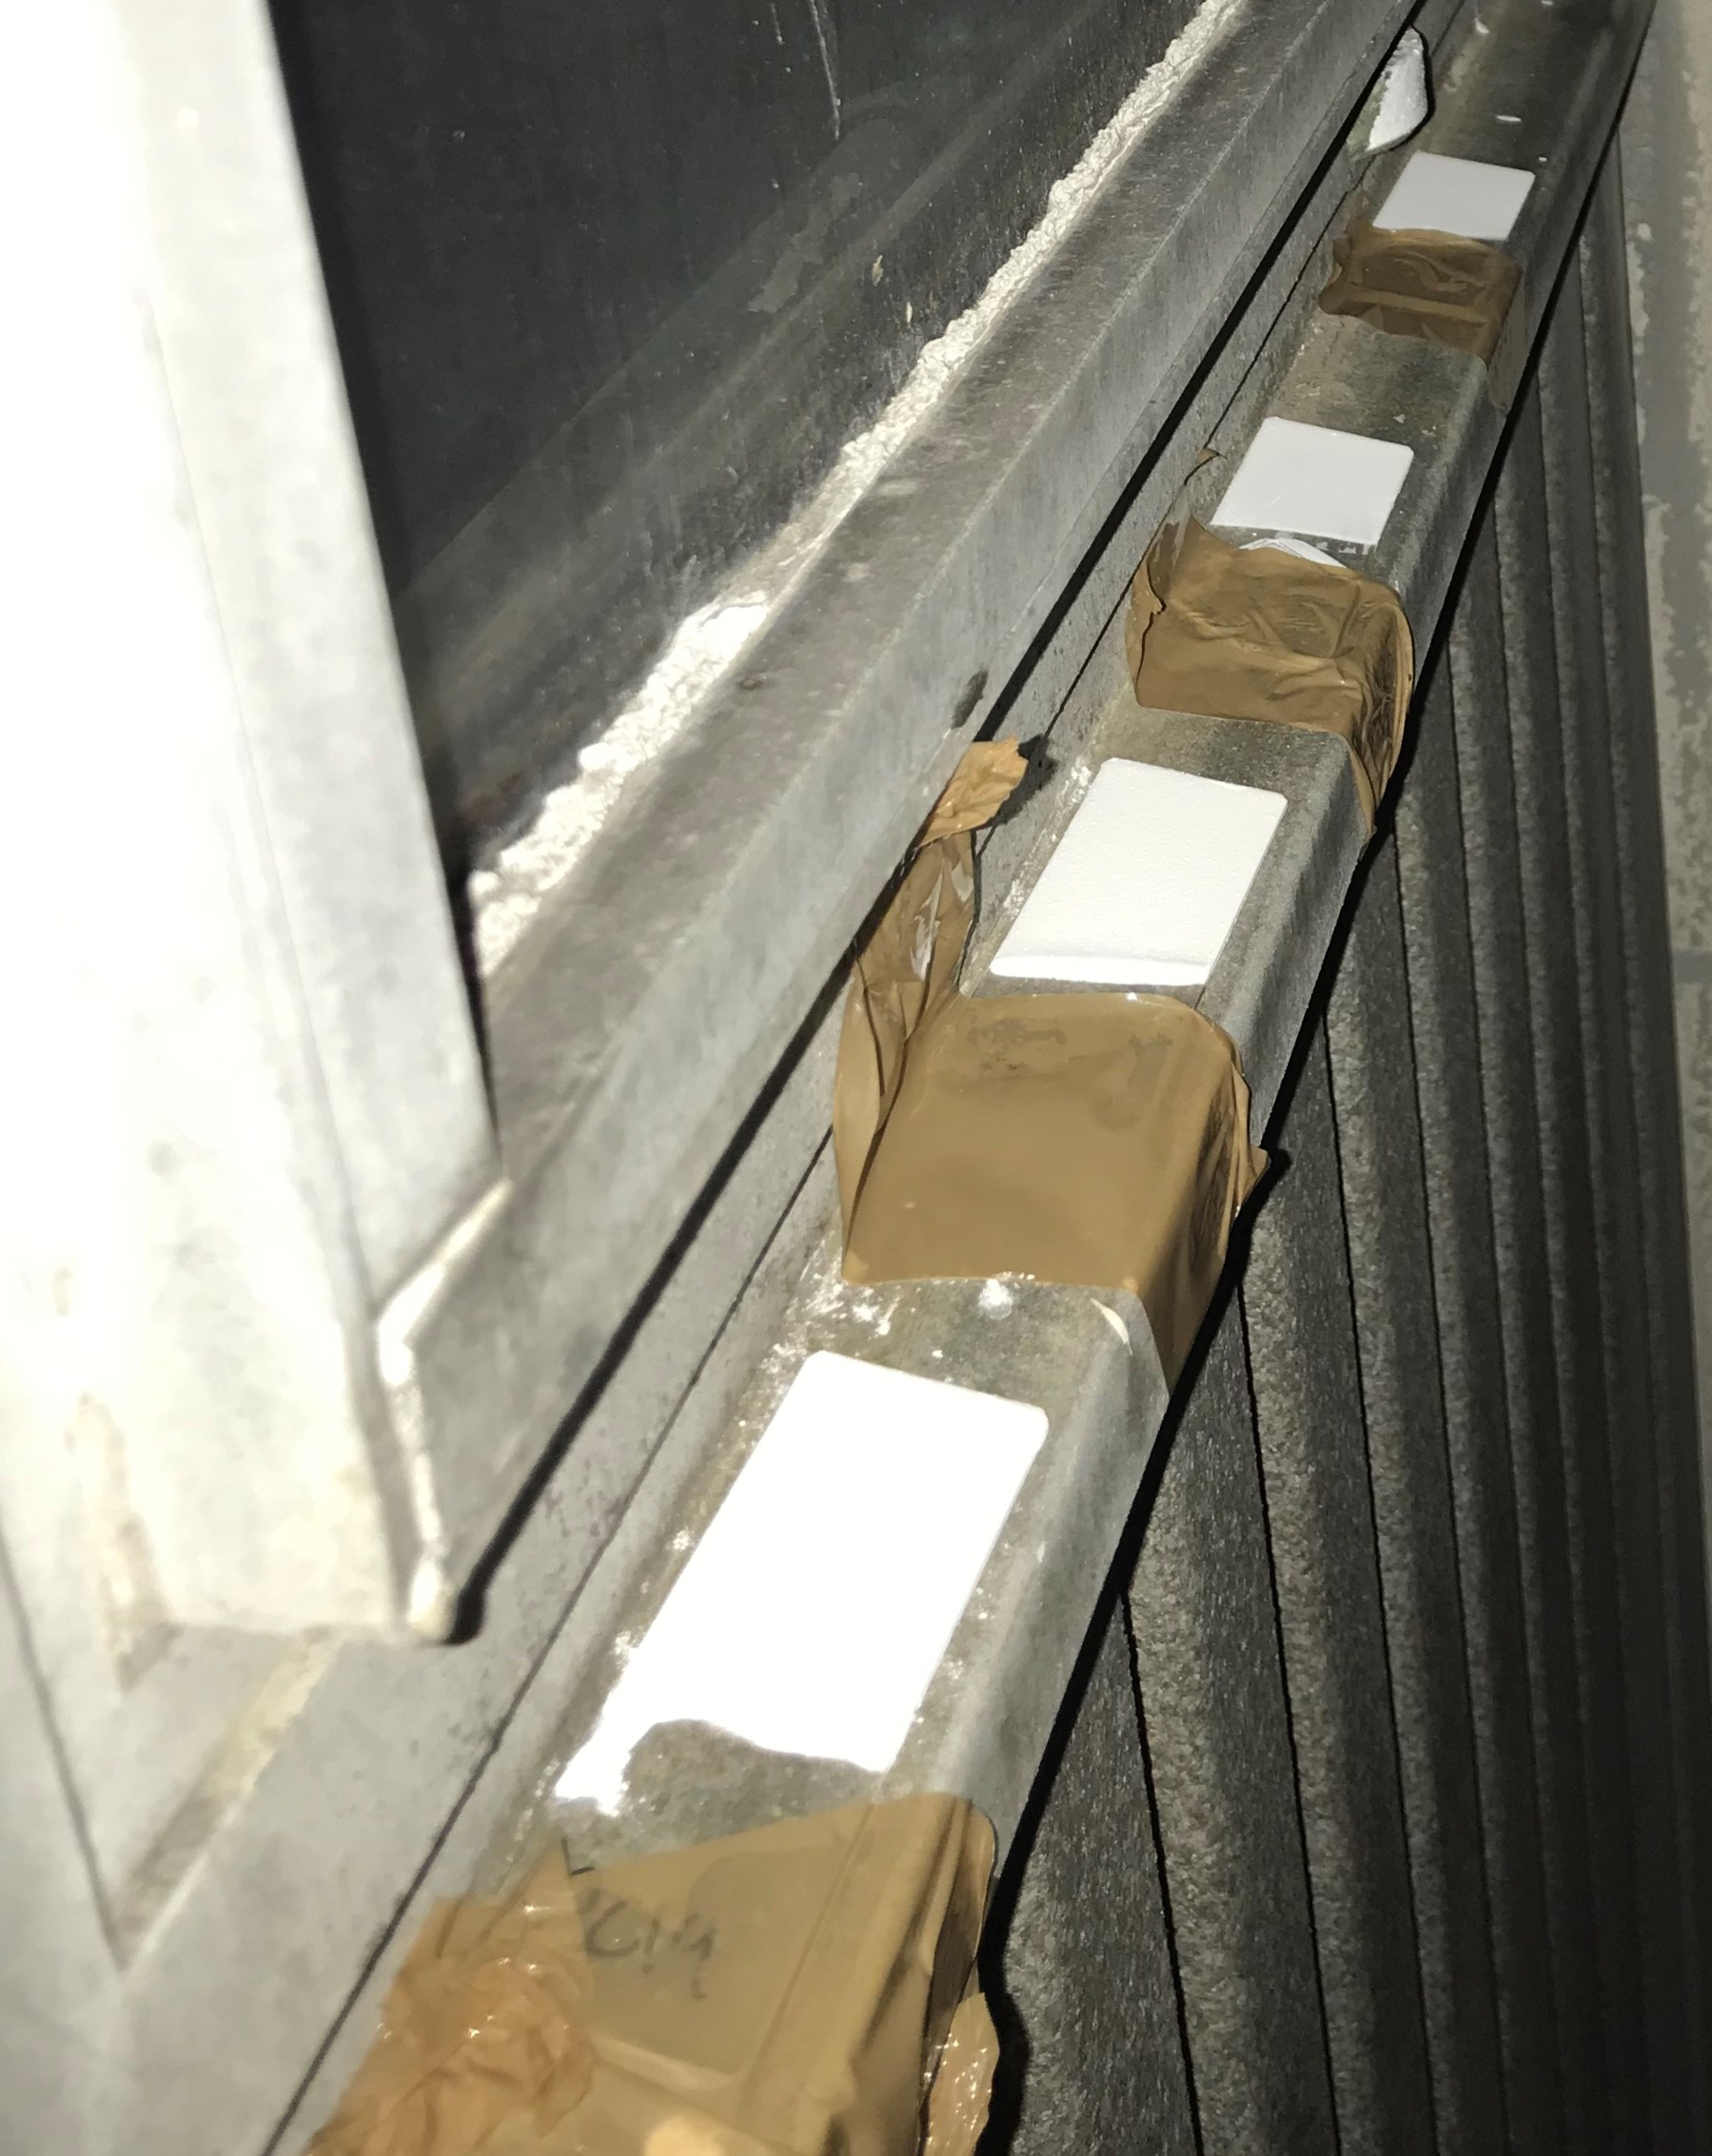
\includegraphics[width=0.09\textwidth]{Sections/Figures/Outdoor.jpg}
  \caption{ A-40-2.5 and B-50-5.5 placed on windowsill at SW7, UK}
  \label{Outdoor}
\end{wrapfigure}


A one-tailed t-test was used to test the hypothesis, at the 95\% significance level that there was no statistical difference before and after the outdoor test. $H_0: \mu_1 = \mu_2$ and $H_1: \mu_1 > \mu_2$. $\nu$ = 4 and so $t_c = 2.132$. Therefore, the null hypothesis was not rejected, and it was concluded that the integrity of both coatings was retained in outdoor conditions.


